\renewcommand{\chapid}{numerics}

% Chapter specific commands:

\newcommand{\LL}{\mathcal{L}}
\newcommand{\UU}{\mathcal{U}}
\newcommand{\FF}{\mathcal{F}}
\newcommand{\VV}{\mathcal{V}}
\renewcommand{\AA}{\mathcal{A}}
\renewcommand{\SS}{\mathcal{S}}
\newcommand{\PP}{\mathcal{P}}
\newcommand{\UUU}{\mathrm{U}}
\newcommand{\FFF}{\mathrm{F}}
\newcommand{\SSS}{\mathrm{S}}
\newcommand{\dual}[1]{*\!\! #1}
\newcommand{\dualt}[1]{*\! #1}
\newcommand{\Risco}{R_{\rm ISCO}}
\newcommand{\sgn}{\mathrm{sgn}}
\newcommand{\CFL}{\mathtt{CFL}}
\newcommand{\ctop}{{\tt cons2prim}}

% Math:

\chapter{Numerical Relativistic Hydrodynamics\chaplabel{numerics}}

This Chapter presents ongoing work with Paul Duffell and Andrew MacFadyen which will be incorporated into a future publication upon the public release of \grdisco, a GRMHD extension to the \disco code written by Paul Duffell.

%%%%%
% Abstract
%%%%%

\section{Chapter Abstract}

We formulate and review the system of equations relevant for astrophysical fluid flow, particularly in a relativistic context.  We develop numerical methods for solving these equations in the finite volume formulation, with a particular focus on schemes which allow for a moving numerical mesh.  These schemes are implemented in \grdisco, a new three dimensional massively parallel general relativistic magnetohydrodynamics code with a moving, shearing mesh.  We run \grdisco\ through a series of tests demonstrating its accuracy and efficacy for many problems of astrophysical fluid dynamics.  \grdisco is freely available at \url{https://github.com/geoffryan/Disco.git}.

%%%%%
%Section 1 - Introduction
%%%%%

\section{Introduction} \sectlabel{intro}

At macroscopic scales the universe can be described as a $3+1$ dimensional Lorentzian manifold with metric tensor $g_{\mu\nu}$ and a number of interacting, dynamical fields.  These fields are governed by an action principle
\begin{equation}
	S = \int d^4x \sqrt{-g} \left( \frac{1}{16\pi} R - \frac{1}{4}F^{\mu\nu}F_{\mu\nu}  + \LL_M\right)\ . \eqlabel{action}
\end{equation}
In \eq{action} $R$ is the Ricci scalar of the metric tensor $g_{\mu\nu}$, $F_{\mu\nu} = \nabla_\mu A_\nu - \nabla_\nu A_\mu$ is the electromagnetic field strength tensor for the electromagnetic four potential $A_\mu$, and $\LL_M$ is the Lagrangian associated with all other matter fields and their interactions.  We will use $\LL_G$ and $\LL_{EM}$ to refer to the first and second terms of \eq{action} respectively.

  The matter fields, $A_\mu$, and $g_{\mu\nu}$ evolve in such a way that $\delta S = 0$.  The resulting Euler-Lagrange equations for $A_\mu$ take the form:
  \begin{align}
  	\nabla_\mu F^{\mu\nu} &= J^\mu \eqlabel{maxwell1} \ , \\
	\text{where } J^\mu &= \frac{\delta \LL_M}{\delta A_\mu}\ .
   \end{align}
   The construction of $F_{\mu\nu}$ is such that it obeys a Bianchi identity $\nabla_{[\mu}F_{\nu\sigma]} = 0$.  This is better stated in terms of the dual tensor $*F_{\mu\nu}$:
     \begin{align}
  	\nabla_\mu *\! F^{\mu\nu} &= 0 \eqlabel{maxwell2} \ , \\
	\text{where } *\! F^{\mu\nu} &= \frac{1}{2}\epsilon^{\mu\nu\sigma\lambda}F_{\sigma\lambda} \ .
   \end{align}
   The Equations \eqrefp{maxwell1} and \eqrefp{maxwell2} together are Maxwell's equations.
   
   Similarly, the Euler-Lagrange equations for $g_{\mu\nu}$ give the Einstein Field Equations:
  \begin{align}
	G_{\mu\nu} &= 8\pi T_{\mu\nu} \eqlabel{einstein} \ , \\
	\text{where } G_{\mu\nu} &= R_{\mu\nu} - \frac{1}{2}g_{\mu\nu} R \ , \\
	\text{and } T_{\mu\nu} &= \frac{-2}{\sqrt{-g}} \frac{\delta}{\delta g^{\mu\nu}}\left(\sqrt{-g}\left( \LL_M + \LL_{EM} \right)\right) \ . \eqlabel{defTmunu}
   \end{align} 
   The Einstein tensor $G^{\mu\nu}$ also obeys a Bianchi identity $\nabla_\mu G^{\mu\nu}=0$. By the Einstein Field Equations \eqrefp{einstein}, the stress-energy tensor $T^{\mu\nu}$ must obey the same identity:
   \begin{equation}
   	\nabla_\mu T^{\mu\nu} = 0 \eqlabel{consSE}\ .
   \end{equation}  
   \eq{consSE} expresses local conservation of energy and momentum.
   
   \subsection{3+1 Splitting of Spacetime}
   
   It can be very useful to split tensors into their space-like and time-like components.  This is referred to as $3+1$ splitting or the Arnott-DeWitt-Misner (ADM) form \citep{ADM}.  We first introduce the unit time-like normal vector $n^\mu$, normal to surfaces of constant time $t$:
   \begin{equation}
   	n_\mu \propto \partial_\mu t\ , \qquad g_{\mu\nu}n^\mu n^\nu = -1\ .
   \end{equation}
   Such a vector can be written as $n_\mu = (-\alpha, 0, 0, 0)$, where the normalization factor $\alpha$ is the \emph{lapse}.  The contravariant components are $n^\mu = (1/\alpha, -\beta^i/\alpha)$ where $\beta^i$ is the \emph{shift}.  A spatial metric $\gamma_{\mu\nu}$ can be constructed by projecting $n^\mu$ out of the metric tensor.  The result is:
   \begin{equation}
   	\gamma_{\mu\nu} = n_\mu n_\nu + g_{\mu\nu}\ .
   \end{equation}
   One can decompose the metric tensor into the 3+1 quantities $\alpha$, $\beta^i$, and $\gamma_{ij}$.  The line element takes the ADM form:
   \begin{equation}
   	ds^2 = -\alpha^2 dt^2 + \gamma_{ij}\left(dx^i + \beta^idt\right)\left(dx^j + \beta^jdt\right)\ .
   \end{equation}
   The inverse metric takes the form:
   \begin{equation}
   	g^{\mu\nu} = \begin{pmatrix} -\alpha^{-2} & \alpha^{-2}\beta^j \\
							\alpha^{-2}\beta^i & \gamma^{ij} - \alpha^{-2}\beta^i \beta^j \end{pmatrix}\ .
   \end{equation}
   A \emph{spatial} vector is any vector $v^\mu$ such that $n_\mu v^\mu = 0$, or equivalently $v^0 = 0$.  A spatial vector has only three independent components: the spatial components $v^i$.  These spatial components may be raised and lowered with the spatial metric $\gamma_{ij}$.  By defining $\gamma \equiv \det \gamma_{ij}$ we can decompose the volume element:
   \begin{equation}
   	\sqrt{-g} = \alpha \sqrt{\gamma} \ .
   \end{equation}
   
\subsection{Matter Content and Hydrodynamics}

   The matter Lagrangian $\LL_M$ and its equations of motion are complicated functions of many interacting fields.  At macroscopic scales the fields can be described as a large number $N \gg 10^{23}$ of discrete interacting particles.  In this work we avoid dealing directly with the particle equations of motion and instead work in the \emph{fluid approximation}.    In this approximation the ensemble of particles is locally described by a number density $n(x)$, a four velocity $u^\mu(x)$, and a temperature $T(x)$.  Symmetries of $\LL_M$ correspond to conservation laws which must still be obeyed in the fluid description.  Of particular use is the conservation of baryon number, which requires the local number density of baryons $n_b(x)$ to obey a continuity equation:
   \begin{equation}
   	\nabla_\mu \left(n_b\ u^\mu\right) = 0 \eqlabel{contnb}\ .
   \end{equation}
  The fluid approximation reduces the description of matter to five degrees of freedom: the number density, the temperature, and the three independent components of the fluid velocity.  The continuity equation \eqrefp{contnb} plus the four equations of energy-momentum conservation \eqrefp{consSE} then provide enough constraints to solve the system so long as it is possible to express the stress-energy tensor $T^{\mu\nu}$ in terms of $n$, $T$, and $u^\mu$ alone, avoiding direct consideration of the material equations of motion.
  
  Consider a gas of particles of mass $m$ in a local rest frame. The gas has mass density $\rho = m n$, thermodynamic pressure $P(n,T)$, and internal energy density $u(n,T)$.  We define the total energy density $e = \rho + u$ and the specific energy density $\eps = u / \rho$.  Relativistic kinetic theory establishes that In a local orthonormal frame the stress-energy tensor has components \citep{RezzollaZanotti}:
  \begin{equation}
  	T^{\hat{\mu}\hat{\nu}} = \begin{pmatrix} e & 0 & 0 & 0 \\
									0 & P & 0 & 0 \\
									0 & 0 & P & 0 \\
									0 & 0 & 0 & P \end{pmatrix}\ .
  \end{equation}
In this frame the metric tensor takes the form $g_{\hat{\mu}\hat{\nu}} = \text{diag}(-1,1,1,1)$ and the four velocity $u^{\hat{\mu}}  = (1,0,0,0)$.  This leads to the unique decomposition $T^{\hat{\mu}\hat{\nu}} = e u^{\hat{\mu}}u^{\hat{\nu}} + P ( u^{\hat{\mu}}u^{\hat{\nu}} + g^{\hat{\mu}\hat{\nu}})$.  This is an equation between tensors, and hence must be true in all frames. Defining the specific enthalpy $h = (e+P)/\rho = 1 + \eps + P/\rho$ we arrive at the stress-energy tensor for a perfect fluid:
\begin{equation}
	T^{\mu\nu}_{gas} = \rho h \ \! u^\mu u^\nu + P g^{\mu\nu} \eqlabel{defTgas}\ .
\end{equation}
The pressure and internal energy are functions of the local density and temperature, which must be determined from the properties of the particular fluid under consideration.  These relationships are referred to as the equation of state of the fluid.  A common equation of state, one assumed throughout this thesis, is the gamma law:
\begin{equation}
	P = (\Gamma - 1)\rho \eps \ , \eqlabel{gammalaw}
\end{equation}
where $\Gam$, a constant, is the \emph{adiabatic index} of the gas under consideration.  Monatomic non-relativistic gases correspond to $\Gam=5/3$, diatomic non-relativistic gases to $\Gam=7/4$, and relativistic gases to $\Gam=4/3$.

\subsection{Electromagnetic Content and MHD}

The field strength tensor $F^{\mu\nu}$ is antisymmetric, $F^{\nu\mu} = -F^{\mu\nu}$, and has six independent components corresponding to the three components each of the electric and magnetic fields $E^\mu$ and $B^\mu$.  Decomposing $F^{\mu\nu}$ into electric and magnetic fields is a frame-dependent procedure.  Elementary electromagnetism teaches us that observers moving with relative velocities will observe different electric and magnetic fields.  The fields in the coordinate frame are defined by:
\begin{align}
	E^\mu = n_\nu F^{\mu\nu} \quad \text{and} \quad B^\mu = n_\nu \dual{F}^{\nu\mu}\ . \eqlabel{defEB}
\end{align}
The electric and magnetic fields are spatial vectors: $n_\mu E^\mu = n_\mu n_\nu F^{\mu\nu} = 0$ due to the antisymmetry of $F^{\mu\nu}$ and $\dualt{F}^{\mu\nu}$. They each have three independent components $E^i$ and $B^i$, totaling to the six components of $F^{\mu\nu}$.  The decomposition of $F^{\mu\nu}$ and $\dualt{F}^{\mu\nu}$ into electric and magnetic fields is:
\begin{align}
	F^{\mu\nu} &= n^\mu E^\nu - n^\nu E^\mu + \eps^{\mu\nu\sigma\lambda}n_\sigma B_\lambda\ , \eqlabel{FEB}\\
	\dualt{F}^{\mu\nu} &= B^\mu n^\nu - B^\nu n^\mu + \eps^{\mu\nu\sigma\lambda}n_\sigma E_\lambda\ .
\end{align}
The four velocity of an observer serves as their local time-like unit vector.  Hence this same decomposition can be done for \emph{any} observer merely by substituting their four velocity $u^\mu$ for $n^\mu$ and renaming the fields, for instance to $e^\mu$ and $b^\mu$.

  We can use \eq{defTmunu} to find the stress energy tensor for the electromagnetic field:
  \begin{equation}
  	T^{\mu\nu}_{EM} = F^{\mu\sigma} F^\nu_\sigma - \frac{1}{4}g^{\mu\nu}F^{\sigma \lambda}F_{\sigma\lambda}\ . \eqlabel{TEMF}
  \end{equation}
  In terms of $E^\mu$ and $B^\mu$ the stress tensor is:
  \begin{equation}
  	T^{\mu\nu}_{\text{EM}} = \left(n^\mu n^\nu + \frac{1}{2}g^{\mu\nu}\right)\left(E^2 + B^2\right) - E^\mu E^\nu - B^\mu B^\nu - \left(n^\mu \eps^{\nu \sigma \lambda \rho} + n^{\nu}\eps^{\mu \sigma \lam \rho}\right)n_\sig E_\lam B_\rho\ . \eqlabel{TEMEB}
  \end{equation}
  In many astrophysical situations the plasma under consideration has very little resistivity: any electric field in the fluid frame $u^\mu$ is quickly neutralized due to motion of electrons.  The length scale on which a plasma may have appreciable net charge density $q$ (and hence electric field) before this screening occurs is the \emph{Debye length} $\lam_{\text{Deb}} \propto \sqrt{T/q}$.  On scales larger than $\lam_{\text{Deb}}$ we can assume the plasma is neutral and has no electric field in the fluid frame.
  
  This is the central assumption of \emph{magnetohydrodynamics} (MHD), and we will restrict our study to astrophysical systems where it holds.  For a fluid (plasma) with four velocity $u^\mu$, we refer to the fluid frame electric and magnetic fields as $e^\mu = u_\nu F^{\mu\nu}$ and $b^\mu = u_\nu\dualt{F}^{\nu\mu}$. The fluid frame fields are not spatial vectors (in the coordinate frame), instead they are orthogonal to the four velocity: $u_\mu e^\mu = u_\mu b^\mu = 0$.  The MHD condition is $e^\mu = 0$.  This simplifies the field strength \eqrefp{FEB} and stress energy \eqrefp{TEMEB} tensors dramatically:
  \begin{align}
  	F^{\mu\nu}_{\text{MHD}} &= \eps^{\mu\nu\sig\lam}u_\sig b_\lam \ , \eqlabel{FMHD} \\
	\dualt{F}^{\mu\nu}_{\text{MHD}} &= b^\mu u^\nu - b^\nu u^\mu \ , \eqlabel{dFMHD} \\
  	T^{\mu\nu}_{\text{MHD}} &=  b^2 u^\mu u^\nu  + \frac{1}{2}g^{\mu\nu} b^2  - b^\mu b^\nu\ . \eqlabel{TMHD}
  \end{align}
    Constructing $B^\mu$ from $b^\mu$ and vice versa is straightforward using the definition \eqrefp{defEB} and the projection tensor $g_{\mu\nu} + u_\mu u_\nu$:
    \begin{align}
    	B^\mu &= w b^\mu - \alpha b^0 u^\mu \ , \\
	b^\mu &= \frac{1}{w}\left(B^\mu + u_\nu B^\nu u^\mu\right) \ ,
    \end{align}
    where $w \equiv -n_\mu u^\mu = \al u^0$ is the fluid Lorentz factor.  Two useful expressions are:
    \begin{align}
    	b^0 &= \frac{1}{\al} u_\mu B^\mu \ , \\
	b^2 &\equiv g_{\mu\nu} b^\mu b^\nu = \frac{1}{w^2}\left(B^2 + \left(u_\mu B^\mu\right)^2\right) \ .
    \end{align}
    We can now write $\dualt{F}^{\mu\nu}_{\text{MHD}}$ in terms of $B^\mu$ and $u^\mu$:
    \begin{equation}
    	\dualt{F}^{\mu\nu}_{\text{MHD}} = \frac{1}{w}\left(B^\mu u^\nu - B^\nu u^\mu\right) \ . \eqlabel{FmunuMHD}
    \end{equation}
    And can finally write the sourceless Maxwell Equations \eqrefp{maxwell2} in MHD:
    \begin{align}
    	\nabla_\mu \left[\frac{1}{w}\left(B^\mu u^\nu - B^\nu u^\mu\right)\right] = 0\ .
    \end{align}
    Writing these equations in terms of coordinate derivatives and splitting off the temporal part, we arrive at four equations: the constraint $\nabla \cdot B = 0$ and the evolution equations for $B^i$:
    \begin{align}
    	\partial_j \left( \sqrt{\gam} B^j \right) &= 0 \ , \eqlabel{divB}\\
	\partial_t \left( \sqrt{\gam} B^i \right) + \partial_j \left(\sqrt{\gam}\left(B^i v^j - B^j v^i\right)\right) &= 0\ . \eqlabel{induction}
    \end{align}
    Lastly we can write down the combined stress-energy tensor for a magnetized perfect fluid in MHD.
    \begin{equation}
    	T^{\mu\nu} = \left(\rho h + b^2\right) u^\mu u^\nu + \left(P + \frac{1}{2}b^2\right)g^{\mu\nu} - b^\mu b^\nu \ . \eqlabel{TmunuGRMHD}
    \end{equation}
    This gives us all the tools we need to begin investigating these flows numerically.

\section{Numerical Solutions to Hyperbolic Equations: The \grdisco\ code}

We have established that an ideal astrophysical plasma will obey the equations of general relativistic magnetohydrodynamics (GRMHD):
\begin{align}
	\nabla_\mu  \rho u^\mu &= 0\ , \eqlabel{GRMHD1}\\
	\nabla_\mu T^{\mu\nu} &= 0\ , \eqlabel{GRMHD2}\\
	\nabla_\mu \dual{F}^{\mu\nu} &= 0\ . \eqlabel{GRMHD3}
\end{align}
In the above $T^{\mu\nu}$ is given by \eq{TmunuGRMHD} and $\dualt{F}^{\mu\nu} = \dualt{F}^{\mu\nu}_{\text{MHD}}$ given by \eq{FmunuMHD}.  These equations all take the form of conservation laws and form a system of non-linear hyperbolic partial differential equations.  The numerical solution of hyperbolic systems of equations is a rich field of numerical analysis.  For our purposes we will focus on \emph{finite volume} schemes.  To do so we must first establish the integral form of Equations (\eqref{GRMHD1}-\eqref{GRMHD3}).  We begin by expressing the covariant derivatives as coordinate derivatives, which put (\eqref{GRMHD1}-\eqref{GRMHD3}) in the form:
\begin{align}
	\partial_\mu \left(\sqrt{-g}\ \! \rho u^\mu\right) &= 0\ , \\
	\partial_\mu\left( \sqrt{-g}\ \!T^{\mu}_\nu\right) &= \frac{1}{2}\sqrt{-g}\ \!T^{\alpha\beta}\partial_\nu g_{\alpha \beta}\ , \\
	\partial_\mu \left(\sqrt{-g}\ \! \dual{F}^{\mu\nu}\right) &= 0\ . \eqlabel{GRMHDcoord}
\end{align}
These equations are each in \emph{conservative} form
\begin{equation}
	\partial_t\ \!\sqrt{-g}\, u + \partial_i\, \sqrt{-g}f^i = \sqrt{-g}\,s \ .
\end{equation}
We call $u$ the conserved variable, $f^i$ the flux, and $s$ the source. The GRMHD system consists of eight such coupled equations which we can index with $a=1,\dots,8$:
\begin{equation}
	\partial_t\ \!\sqrt{-g}\, u_a + \partial_i\, \sqrt{-g}f^i_a = \sqrt{-g}\,s_a \ . \eqlabel{hyperbolicsystem}
\end{equation}
This is called the Valencia formulation of GRMHD \citep{Marti91, Banyuls97, Font08}.  It has been implemented in several codes, for instance \citealt{HARM} and \citealt{Duez05}.

Each of these equations is a conservation law for $u_a$.  The fluxes $f^i_a$ and sources $s_a$ in general depend non-linearly on the entire set of $u_a$'s.  In fact, in GRMHD the functions $f^i_a(u_a)$ and $s_a(u_a)$ have no known exact form.  Instead, $u_a$, $f^i_a$, and $s_a$ are all known only as functions of the \emph{primitive} variables $\PP_a$. 

In GRMHD we often take $\PP_a = (\rho, P, v^1, v^2, v^3, B^1, B^2, B^3)$ where $v^i = u^i/u^0$.  \grdisco\ also can use $u_i$ instead of $v^i$ and $T$ instead of $P$.  It will be stated when either of these alternatives are used. Once a choice of $\PP_a$ has been made, the conserved variables, fluxes, and sources terms may all be calculated.

There is some freedom in the choice of conserved variables.  In particular, any linear combination of the variables in $(\eqref{GRMHD1}-\eqref{GRMHD3})$ will also be conserved.  We take $u_a = (D, T^0_1, T^0_2, T^0_3, \tau_U, B^1, B^2, B^3)$ where $D = \rho u^0$, $\tau_U \equiv -U_\mu T^{0\mu}-D$, and $U^\mu$ is an exactly known timelike unit vector.  The energy variable $\tau_U$ is a generalization of the variable $\tau = -n_\mu T^{\mu0} - D$ used in many codes \citep{HARM, Duez05}.

\subsection{Finite Volume Form}
Our numerical scheme relies on the integral form of \eq{hyperbolic system}, which is easier to stabilize and implement in non-Cartesian geometries.  

Consider a rectangular control volume $\VV$ spanning $x^1\in [x^1_-, x^1_+]$,  $x^2\in [x^2_-, x^2_+]$, and  $x^3\in [x^3_-, x^3_+]$.  Let $dV=\sqrt{-g}dx^1dx^2dx^3$.  We will assume the volume can stretch in the $x^1$ direction and let $x^1_\pm = x^1_\pm(t)$.  The mass of $u_a$ in $\VV$ is:
\begin{equation}
	\UUU_a = \intop_\VV dV\, u_a = \int \limits_{x^1_-(t)}^{x^1_+(t)} \int \limits_{x^2_-}^{x^2_+} \int \limits_{x^3_-}^{x^3_+} dx^1dx^2dx^3 \sqrt{-g}\, u_a\ .
\end{equation}
The time derivative of $\UUU_a$ depends on $\partial_t u_a$ and $V^1_\pm \equiv d x^1_\pm /dt$:
 \begin{equation}
 \frac{d}{dt}\UUU_a = \int \limits_{x^1_-}^{x^1_+} \int \limits_{x^2_-}^{x^2_+} \int \limits_{x^3_-}^{x^3_+} dx^1dx^2dx^3 \partial_t\left(\sqrt{-g}\, u_a\right) + \left .  \int \limits_{x^2_-}^{x^2_+} \int \limits_{x^3_-}^{x^3_+} dx^2dx^3 \sqrt{-g}\, V^1  u_a\right |^{x^1_+}_{x^1_-}\ .
 \end{equation}
 Let $dA_1 =\sqrt{-g} dx^2 dx^3$, $dA_2 = \sqrt{-g}dx^1 dx^3$, and $dA_3 = \sqrt{-g}dx^1dx^2$.   We will use $\AA_{i\pm}$ to refer to the faces $\VV$, surfaces of constant $x^i_\pm$. Inserting \eq{hyperbolicsystem} for $\partial_t \sqrt{-g} u_a$ and using Stoke's Theorem allows us to arrive at the integral equation:
 \begin{equation}
	\frac{d}{dt} \UUU_a = -\left .\intop_{\AA_1}dA_1 \left(f^1_a - V^1u_a\right) \right |_{x^1_-}^{x^1_+} -\left .\intop_{\AA_2}dA_2 f^2_a \right |_{x^2_-}^{x^2_+} -\left .\intop_{\AA_3}dA_3 f^3_a \right |_{x^3_-}^{x^3_+} +  \intop_\VV dV\, s_a\ . \eqlabel{integralform}
\end{equation}
The volumes and areas of cells and faces are defined as:
\begin{align}
	\Delta V &= \intop_\VV dV \ , \\
	\Delta A_{i\pm} &= \intop_{\AA_{i\pm}} dA_i \ .
\end{align}
This allows us to consider the averaged quantities:
\begin{align}
	\UU_a &= \frac{1}{\Delta V} U_a\ , \\
	\FF^{i\pm}_a &= \frac{1}{\Delta A_{i\pm}}  \intop_{\AA_{i\pm}} dA_i\, f^i_a \ ,  \\
	\widehat{u}_a^{i\pm} &=  \frac{1}{\Delta A_{i\pm}}    \intop_{\AA_{i\pm}} dA_i \, u_a\ , \\
	\SS_a &= \frac{1}{\Delta V} \intop_\VV dV\, s_a\ .
\end{align}
Letting the index $p=  1+, 1-, \dots, 3-$ denote the six faces of $\VV$ we can write \eq{integralform} in \emph{finite volume} form:
\begin{equation}
\frac{d}{dt}\left( \UU_a \Delta V\right) = -\sum_{p}\Big[\sgn(p)\big(\FF^{p} - V^{p} \widehat u_a^{p}\big)\Delta A_{p}\Big] + \SS_a \Delta V\ . \eqlabel{FVform}
\end{equation}
This is an exact equation for the rate of change for the mass of $u_a$ in volume $\VV$, equal to the sum of the face averaged fluxes (adjusted for the face movement) and the volume integrated source function.  The finite volume (FV) numerical schemes directly solve this equation for $\UU_a$ given an approximate scheme for evaluating $\FF_a$.

\subsection{The \grdisco\ Grid}

\grdisco\ solves the GRMHD equations in finite volume form \eqrefp{FVform} on a three dimensional shearing mesh.  Although the code is written to use general coordinates $x^\mu$, the reconstruction and source term integration are optimized for a cylindrical geometry $x^i = (r, \phi, z)$.  In describing the code, these coordinates will often be used.  The method of solution and grid structure are all shared with \disco\ \citep{Duffell16}, and are summarized below.  The GRMHD-specific routines are an extension to the basic \disco\ code base.

The domain of the calculation is first split in the $r$ and $z$ directions, forming an $N_r\times N_z$ Cartesian grid of annuli.  The radial and vertical faces may in principle have arbitrary spacing, although in practice vertical faces are spaced at regular (linear) intervals and the radial faces are spaced regularly in $r$ or $\log r$.  Each annulus is divided into $N_\phi(r,z)$ cells.  $N_\phi$ may, and often does, change with $r$ and $z$ so adjacent annuli may not have the same number of cells.  The faces between neighbouring cells within an annulus can move, allowing cells to stretch, shrink, or simply transit along their annulus.  The velocity of the radial and vertical faces are all identically zero.  The total number of cells is $N$.

The numerical solution to \eq{hyperbolicsystem} in finite volume form \eqrefp{FVform} at time $t$ is represented by a value for the mass $(\UUU_a)_q$ in each cell $q=1,\dots,N$.  We follow the approach of the \emph{method of lines}, first discretizing in space and constructing a coupled system of ordinary differential equations which can be numerically integrated by standard techniques.

\grdisco\ is second order in space, the local truncation error scales as $(\Delta x)^2$.  At this order, cell averages of a quantity are equal to their value at the cell centers: $(\UU_a)_q = u_a(x_q)$ and $(\SS_a)_q = s_a(x_q)$ where $x_q$ is the center of cell $q$.  Since the mesh can shear azimuthally cells on adjacent annuli do not line up and cells will in general have more than six neighbours.  We will index the faces (the surface segment shared by a cell and its neighbour) of cell $q$ as $p_q$ and following \eq{FVform} use $\sgn(p_q)$ to denote whether surface is oriented inwards or outwards.  This allows us to write:
\begin{equation}
	\frac{d}{dt} \left(\UUU_a\right)_q = \sum_{p_q} \Big[\sgn(p_q)\big(\FF^{p_q}(u_L,u_R) - V^{p_q} \widehat u_a^{p_q}(u_L,u_R)\big)\Delta A_{p_q}\Big] + s_a(u_a) \Delta V\ , \eqlabel{numFVform}
\end{equation}
where $u_L$ and $u_R$ are interpolations of local fluid variables to the left and right sides of the face $p_q$ respectively.  Each $u_K$, $K=L,R$, is a function of a local stencil of $(u_a)_q$'s.  In this way the evolution of the $(\UUU_a)_q)$ are coupled, with the degree of coupling dependent on the order of the scheme.  \eq{numFVform} is a coupled system of first order ordinary differential equations in the $8\times N$ variables $(\UUU_a)_q$.

Constructing appropriate $u_K$ at a given spatial order is called \emph{reconstruction} and considered in \sect{reconstruction}.  Calculating an appropriate value for $\FF(u_L, u_R)$ is done in \grdisco\ by an approximate Riemann solver, this procedure is detailed in \sect{riemann}.  The time evolution of \eq{numFVform} is covered in \sect{timeevolution}.

\subsection{Time Evolution}
\sectlabel{timeevolution}
In \grdisco\ the numerical grid also evolves: the cell volumes $\Delta V_q$ and face areas $\Delta A_p$ are not constant.  The full set of data are then the $8N$ fluid variables $(U_a)_q$ and the azimuthal face positions $\phi_{q+1/2}(t)$, where $q+1/2$ denotes that this corresponds to the forward (increasing $\phi$) face of cell $q$.  The face velocity is set by the current fluid and grid variables by a function $V^\phi$:
\begin{equation}
	\frac{d}{dt} \phi_{q+1/2} = V^\phi((u_a)_{q'}, \phi_{q'+1/2}) \ . \eqlabel{faceMovement} 
\end{equation}
We use $Z = \{ (U_a)_q, \phi_{q+1/2} \}$ to denote the collection of all $9N$ dynamic variables.  Its time derivative is denoted $L$:
\begin{equation}
	\frac{d}{dt} Z = L(t, Z)\ . \eqlabel{Zevol}
\end{equation}
This equation may be integrated numerically by Runge-Kutta (RK) methods.  The entire array of $Z$ is evolved over a series of discrete time intervals $\Delta t^n$, where $t^{n+1} = t^n + \Delta t^n$. We denote $Z^n = Z(t^n)$.  \grdisco's first order time evolution algorithm is the forward Euler scheme:
\begin{equation}
	Z^{n+1} = Z^n + \Delta t^n L(t^n, Z^n) \ . \eqlabel{fe}
\end{equation}
The second order algorithm is the total variation diminishing (TVD) RK2 scheme \citep{Gottlieb98}:
\begin{align}
	Z^{(1)} &= Z^n + \Delta t^n L(t^n, Z^n) \\
	Z^{n+1} &= \frac{1}{2}Z^n + \frac{1}{2}\left(Z^{(1)} + \Delta t^n L(t^{n+1}, Z^{(1)}) \right) \ . \eqlabel{rk2}
\end{align}
These explicit integration schemes are subject to the Courant--Friedrichs--Lewy (CFL) condition to ensure their stability \citep{CFL28}.  By this condition the timestep must be shorter than the smallest sound crossing time of a cell.  Denoting the minimum and maximum wavespeeds in the direction $i$ as $\lambda^{i\pm}$, this gives for a general coordinates:
\begin{equation}
	\Delta t < \Delta t_{\mathrm{max}} = \underset{i,q}{\min}\left( \frac{x^i_+ - x^i_-}{\left |\lambda^{i\pm} - V^{i\pm}\right |} \right)\ . \eqlabel{CFL}
\end{equation}
We adhere to the CFL condition by calculating $\Delta t_{\mathrm{max}}$ at the beginning of each time step and setting $\Delta t^n = \CFL\ \Delta t_{\mathrm{max}}$, where $\CFL \in [0,1]$.  In $d$ dimensions typically $\CFL < 1/d$ to ensure stability \cite{Toro}.  We refer to $\CFL$ as the CFL number.

  We see here the first advantage of the moving mesh, the effective wave propagation speed is not $\lambda^i$ but $\lambda^i - V^i$.  For supersonic flows $\lambda^{i\pm}$ is large and dominated by the fluid velocity.  If $V^i$ is chosen to be near the fluid velocity then $\lambda^{i\pm} - V^i$ will be small, $\OO (c_s)$, and $\Delta t_{\mathrm{max}}$ will be larger than otherwise possible.  This allows a moving mesh code to simulate to the same final time with far fewer time steps than a fixed mesh code and can drastically improve efficiency.

\subsection{Reconstruction}
\sectlabel{reconstruction}

To compute the intercell fluxes $\FF^p(u_L,u_R)$, the states $u_L$ and $u_R$ must first be determined.  Without loss of generality we can consider a single cell $q$ and one of its faces $\AA$.  If $\AA$ is located on the leading (increasing $x^i$) side of $q$ the interpolation will produce a $u_L$.  If $\AA$ is located on the trailing (decreasing $x^i$) side of $q$ the interpolation will produce a $u_R$.  We will refer in general to the interpolated value as $u_K$, understanding $K=L$ or $R$.

\grdisco\ uses \disco's interpolation method, documented thoroughly in \citep{Duffell16}.  We will simply quote the results here.

Interpolation is performed on the primitive quantities $(\PP_a)_q$.  If required the conserved variables $u_a$ may always be calculated from $\PP_a$.

A first order scheme is constructed by treating the numerical solution as piecewise constant in every cell.  This is the Piecewise Constant Method (PCM), and produces the simple relationship:
\begin{equation}
	\PP_K = (\PP_a)_q\ .
\end{equation}
In this scheme the flux through a face depends only on the fluid variables immediately neighbouring the face.

A second order scheme is constructed by treating the numerical solution as piecewise linear in every cell.  This is the Piecewise Linear Method (PLM), and requires the calculation of a gradient $\langle \partial_i \PP_a \rangle_q$ of the fluid variables in cell $q$.  Given this gradient, the coordinates of the cell center $x^i_q$, and those of the face center $x^i_f$ we calculate $u_K$ by linear interpolation:
\begin{equation}
	\PP_K = (u_a)_q + \langle \partial_i \PP_a \rangle_q (x^i_f - x^i_q)\ . \eqlabel{PLM}
\end{equation}
The gradient $\langle \partial_i \PP_a \rangle_q$ is a \emph{slope limited} gradient and not equal to the second order accurate cell-centered numerical gradient that one may expect.  The cell centered gradient in fact introduces instabilities near discontinuities that wreck the numerical solution \citep{vanLeer74}.  The solution is to sacrifice second order accuracy near discontinuities by reverting locally to a first order scheme.  When combined with a suitable time evolution scheme such a method is called \emph{total variation diminishing} (TVD).

Reversion to first order is done through a \emph{slope limiter}, a non-linear function of the second order and first order gradients that returns a suitable slope limited numerical gradient.  In \disco we use the Generalized Minmod (GMM) limiter \citep{vanLeer79}, parameterized by a parameter $\theta \in [1,2]$ we refer to as the PLM parameter.  This limiter interpolates between the Minmod (MM) limiter at $\theta=1$ and the Monotonized Central (MC) limiter at $\theta=2$.  The MC limiter is less diffusive than the MM limiter but also more aggressive and prone to instability.  We usually take $\theta=1.5$.  

For details on the specific implementation of the GMM limiter and how gradients are calculated on the shearing mesh see \cite{Duffell16}.

\subsection{Riemann Solvers}
\sectlabel{riemann}

\discogr\ is a \emph{Godunov} code, it calculates intercell fluxes $\FF_a$ by (approximately) solving Riemann problems on each face with initial conditions given by interpolating fluid variables $u_L$ and $u_R$ (or $\PP_L$ and $\PP_R$) from the cell centers.  Godunov schemes have been shown to be highly robust and accurate, particularly in the presence of shock waves.  

We approximate the solution near a particular face as plane parallel and only consider variation in the direction normal to the face.  This makes the problem essentially one dimensional with a piecewise constant initial condition, variables take values $u_L$ to the left of the interface and values $u_R$ to the right.  This is precisely the Riemann problem. In some cases it can be solved exactly, but in numerical codes often approximate Riemann solvers are used.  Approximate solvers are more efficient and can be very accurate.

The desired output from the Riemann solver is the flux $\FF_a$ and fluid state $\widehat{u}_a$ across a face which has velocity $V$. Approximate Riemann solvers capture key elements of the exact Riemann solution. Firstly the solution is self-similar, it only depends on $x^i/t$ (assuming the $x^i$ coordinate is normal to the face).  Second, the solution takes the form of several waves of constant finite speed $\lambda_a$.  There can be at most as many waves as there are equations in the system being solved.  The Rankine--Hugoniot conditions must be satisfied over every discontinuous wave.  Lastly, all Riemann are upwinded: the solution for $x^i/t < \lambda^-$, where $\lambda^-$ is the smallest wave speed, is $\widehat{u}_a = u_L$ and $\FF_a = \FF_L = f(u_L)$.  If $x^i/t >\lambda^+$, where $\lambda^+$ is the largest wave speed, then $\widehat{u}_a = u_R$ and $\FF_a = \FF_R = f(u_R)$.

Every fluid element has the ability to launch a series of waves of speed $\lambda_a$ called \emph{characteristics}.  This is most easily seen in the quasi-linear form of \eq{hyperbolicsystem} expressed in a local orthonormal frame:
\begin{equation}
	\partial_t u_a + \left(\frac{\partial f^i_a}{\partial u_b}\right)\partial_i u_b = s_a\ . \eqlabel{quasilinear}
\end{equation}
The matrix $\partial f^i_a / \partial u_b$ is the \emph{flux Jacobian}.  The characteristic wave speeds $\lambda_a$ are the eigenvalues of the flux Jacobian, one could diagonalize \eqlabel{quasilinear} which would result in a series of uncoupled advection equations with velocity $\lambda_a$ \citep{Leveque97}.  A system of equations is hyperbolic if all the $\lambda_a$ are real and finite.  The details of the possible wave speeds $\lambda_a$ and the physical states they connect is referred to as the characteristic structure of the system.

\discogr\ can use three Riemann solvers: HLL, HLLC, and HLLD.  All take as input the left and right fluid states $u_L$ and $u_R$ and the fastest wave speeds $\lambda^\pm$ defined as:
\begin{align}
	\lambda^+ &= \max\left( \lam_a(u_L), \lambda_a(u_R)\right)\ , \\
	\lambda^- &= \min\left( \lam_a(u_L), \lambda_a(u_R)\right)\ .
\end{align}

The Harten--Lax--van Leer (HLL) solver is the simplest approximate Riemann solver and requires no other knowledge of the characteristic structure of the system \citep{HLL}.  It defines a single average state $(u_{\rm HLL}, \FF_{\rm HLL})$ which lies between $\lam^-$ and $\lam^+$.  Both $u_{\rm HLL}$ and  $\FF_{\rm HLL}$ are determined uniquely by the Rankine--Hugoniot conditions:
\begin{align}
	u_{\rm HLL} &= \frac{\lam^+ u_R - \lam^- u_L - \FF_R + \FF_L}{\lam^+ - \lam^-}\ , \\
	\FF_{\rm HLL} &= \frac{\lam^+ \FF_L - \lam^- \FF_R +\lam^+\lam^-\left(u_R-u_L\right)}{\lam^+ - \lam^-}\ . \\
\end{align}
Averaging over the entire intermediate state, the HLL Riemann solver is the most diffusive and also the most stable.  

For GRHD problems, where $B^i = 0$, \grdisco\ can use the relativistic HLLC solver \citep{Toro94, Mignone05}.  This three wave solver introduces a contact wave with speed $\lam^*$ between $\lam^\pm$ over which the normal velocity must be continuous.  This solver is very accurate and preserves contact discontinuities exquisitely, particularly when combined with mesh motion.

For GRMHD problems \grdisco can use the relativistic HLLD solver \citep{HLLD,Mignone09}.  In this solver the fastest wave speeds correspond to the fast Alfv\'{e}n waves.  There are four intermediate states, separated by the magnetosonic waves and a central contact discontinuity.  When combined with constrained transport and the moving mesh the HLLD solver provides fantastic magnetic field advection with very little diffusion.  In Newtonian simulations HLLD has been found to greatly aid in resolution of the magneto-rotational instability \citep{Sorathia12}.

\subsection{Primitive Variable Recovery: \ctop}
\sectlabel{cons2prim}

In GRMHD and even GRHD there is no exact expression for $f_a$ and $s_a$ in terms of $u_a$.  Rather, primitive variables $\PP_a$ must be used as a go-between. Whenever the conserved variables $\UUU_a$ are updated the relationships $\UUU_a = u_a(\PP) \Delta V$ must be inverted to find the corresponding $\PP_a$.  These can then be used to evaluate $f_a$ and $s_a$ as necessary.

The algorithm which recovers primitive variables often called \ctop.  \grdisco\ has two different \ctop\ routines implemented, a GRHD solver which assumes $B^i=0$ and a more generic GRMHD solver.  Both solvers use the values of $\PP_a$ from the last time step as initial values in an iterative scheme.  

The GRHD solver is adapted from \citet{Duez05} and requires the solution of a quartic equation in $w-1$, where $w = -n_\mu u^\mu$ is the fluid Lorentz factor.  This is done via a Newton-Raphson scheme, which is found to be somewhat more efficient than an exact quartic solver.  Expressing the equation in terms of $w-1$ instead of $w$ (as used in \citet{Duez05}) reduces truncation error in slow flows where $w \approx 1$.

In GRMHD \grdisco\ uses the primitive velocities $u_i$ instead of $v^i$.  This guarantees that all possible primitive states $\PP_a$ correspond physical states.  This is not the case with $v^i$, which are bounded from above to prevent super-luminal velocities.  Aside from this alteration, the GRMHD \ctop\  is a direct implementation of the Noble 2D scheme \citep{Noble06}.  This scheme uses Newton-Raphson to solve a coupled set of equations for $v^2 = \gamma^{ij}u_i u_j / w^2$ and $\eta = w h$.  Both this and the GRHD scheme currently require a gamma law equation of state \eqrefp{gammalaw}, although extensions to generic equations of state are well documented should the need to implement them arise.

\subsection{The $\tau_U$ Energy Variable: Breaking Up With The Coordinate Basis}

By convenience, both indices of the stress energy tensor $T^{\mu\nu}$ are usually assumed to live in the same coordinate basis.  This is essential, for instance, to use the symmetry $T^{\mu\nu} = T^{\mu\nu}$.

Numerically, we have found it is advantageous to consider the mixed rank tensor $T^\mu_\nu$.  In this form the symmetrical nature of ${\bf T}$ is not manifest, but its conservation law takes on a particularly nice form when expressed in coordinate derivatives:
\begin{equation}
	\partial_\mu \sqrt{-g} T^\mu_\nu = \frac{1}{2}\sqrt{-g}T^{\alpha}{\beta}\partial_\nu g_{\alpha \beta}\ .
\end{equation}
In this form, the source term of the equation for $T^0_\nu$ is 0 if $\partial_\nu g_{\alpha \beta} = 0$.  This explicitly builds translational killing vectors into our numerical schemes if we take the conserved quantities to be $T^0_\nu$ and not $T^{0\nu}$, for instance.  This usage of $T^\mu_\nu$ is more akin to the standard construction in which the stress energy tensor is introduced where the $\mu$'th $\nu$'th component of ${\bf T}$ corresponds to the flux in the $\mu$'th direction of the $\nu$'th component of momentum.  In this construction the first and second indices of ${\bf T}$ correspond physically to very different objects.

A priori there is no reason to assume the basis in which we identify the components of the momentum is the same in which we are expressing fluxes.  Fluxes, corresponding to the upper index of $T^\mu_\nu$, are for our numerical purposes oriented along coordinate surfaces, and hence are always expressed in the coordinate basis.  The momentum components, however, may be expressed in any basis we like.  

The energy variable $\tau$ already does this, in fact, by projecting ${\bf T}$ along the timelike normal: $\tau = -n^\nu T^0_\nu - D$.  We have found it very beneficial to consider energy variables defined in a different basis altogether.  Only speaking of the energy equation, one simply needs to specify a timelike unit vector to project against ${\bf T}$.  For some such vector $U^\mu$ we have $g_{\mu\nu}U^\mu U^\nu = -1$ and can write the energy equation as:
\begin{align}
	\nabla_\mu \left( -U_\nu T^{\mu\nu}\right) &= -T^{\mu\nu}\nabla_\mu U_\nu \\
\implies \quad	\partial_\mu \sqrt{-g} \left(-U_\nu T^{\mu\nu}\right) &= -\frac{1}{2}\sqrt{-g}T^{\mu\nu}U^\sig\partial_\sig g_{\mu\nu} - \sqrt{-g}T^\mu_\nu \partial_\mu U^\nu \eqlabel{UTmunu}
\end{align}
So long as $U^\mu(x^\al)$ is known exactly the derivatives $\partial_\mu U^\nu$ can be calculated and \eq{UTmunu} is a good first order conservation law.  The conserved quantity defines our variable energy variable $\tau_U = -U^\nu T^0_\nu - D$.

Although somewhat complicated, picking a good $U^\mu$ can simplify a problem immensely when the flow is supersonic.  This is because projecting onto $U^\mu$ is equivalent to measuring the energy in a frame moving with four velocity $U^\mu$.  If $U^\mu$ can be chosen to be close to the fluid velocity, then $\tau_U$ will be dominated by the internal energy density as the kinetic energy density is zero in the co-moving frame.  This greatly aids in primitive variable inversion as it increases the numerical precision of the recovered internal energy by several orders of magnitude.

A particularly useful $U^\mu$ for thin disks is a congruence of equatorial Keplerian geodesics $U^\mu_{geo}$.  This velocity field is the steady state solution to the equations of motion for cold particles, and as such is very close to the velocity field of thin accretion disks.  Inside the ISCO the four velocity is plunging with constant $U_\phi$ and $U_0$.  The interior $U^r$ can then be determined from the four velocity normalization. To smoothly match with the exterior Keplerian solution $U_\phi$ and $U_0$ must match the Keplerian values at the ISCO.  In the Schwarzschild metric in Kerr-Schild coordinates this takes the form:
\begin{align}
	U^0_{geo} &= \left \{ \begin{matrix} \frac{2\sqrt{2}/3}{1-2M/r} & r < 6M \\
						\frac{1}{\sqrt{1-3M/r}} & r > 6M \end{matrix} \right . , \nonumber \\
	U^r_{geo} &= \left \{ \begin{matrix} -\frac{1}{3}\sqrt{\frac{6M}{r}-1} & r < 6M \\
						0 & r > 6M \end{matrix} \right . , \nonumber \\
	U^\phi_{geo} &= \left \{ \begin{matrix}  \frac{2 \sqrt{3} M}{r^2} & r < 6M \\
						\sqrt{\frac{M/r^3}{1-3M/r}} & r > 6M \end{matrix} \right . . \eqlabel{Ugeo}
\end{align}
The same calculation can be carried out in the equatorial Kerr metric, bearing similar but far more complicated results.  Using this $U^\mu_{geo}$ frame to measure the fluid energy is essential for stably evolving high mach number accreting flows, as shown in \sect{test:kep}.  This frame was put to practical effect in studying minidisks, which will be discussed further in \chap{minidisk}.

\subsection{Constrained Transport}
\sectlabel{constrainedTransport}

Our solution method, so far, has neglected one component of the induction equation \eqrefp{GRMHD3}:
\begin{equation}
	\nabla_\mu \dual{F}^{\mu\nu} = 0\ .
\end{equation}
The $\nu=1,2,3$ components of \eq{GRMHD3} are evolution equations for $B^1, B^2, B^3$ and are part of the hyperbolic system.  The fourth component, $\nu=0$, is a constraint equation which applies on all time slices: $\vec{\nabla}\cdot \vec{B} = 0$, and is not part of the hyperbolic system.

Preserving this constraint numerically is vital to ensuring a stable and accurate evolution \citep{Brackbill80}.  Unfortunately any naive evolution scheme will unavoidably grow $\vec{\nabla}\cdot \vec{B}$ over time. Algorithms designed to evolve the $B^i$ while maintaining the constraint have been the subject of study for a number of years \citep{Evans88,Dai98,Ryu98,Balsara99,Toth00}.  In \grdisco\ we enforce $\vec{\nabla}\cdot \vec{B} = 0$ by implementing \emph{constrained transport} (CT) \citep{Evans88}.  \citet{Duffell16} has a thorough discussion explaining the advantages of CT over other schemes on the \disco\ mesh.

Since electromagnetism is already a relativistic theory, the Newtonian MHD constrained transport implementation in \disco\ can be used for GRMHD with virtually no modification \citep{Duffull16}.  Here we summarize the important features in the language of GRMHD, which should serve as a guide to the \grdisco\ implementation.

The basic idea of CT is that the natural way to formulate MHD is in terms of conserved magnetic fluxes: $\Phi = \int \vec{dA}\cdot \vec{B}$. The flux $\Phi$ obeys a natural conservation law, related to the conservation of magnetic field lines.  This is a lower dimensional conservation law: conserved variables live on faces and are transported through edges, as opposed to the conservation laws considered so far where conserved variables live in cells and are transported through faces.  Forcing the induction equation into a volume conservative form introduces a redundant description which necessitates the $\vec{\nabla}\cdot \vec{B} = 0$ constraint.  A conservation law written in terms of $\Phi$ has no redundancy and no extra equations.

To be definite, we will first consider the flux $\Phi_1$ through a face $\AA_1$.  $\AA_1$ is a surface of constant $x^1$ bounded by $x^2_\pm$ and $x^3_\pm$, we allow $x^1$ to depend on time, $x^1 = x^1(t)$, and denote $V^1 = d x^1/dt$.  This surface will be representative of the constant $\phi$ faces in \grdisco.

The flux is:
\begin{equation}
	\Phi_1 = \int \limits_{x^2_-}^{x^2_+} \int \limits_{x^3_-}^{x^3_+} dx^2 dx^3 \sqrt{\gam} B^1\ .
\end{equation}
The time derivative of this flux is:
\begin{equation}
	\frac{d}{dt}\Phi_1 = \int \limits_{x^2_-}^{x^2_+} \int \limits_{x^3_-}^{x^3_+} dx^2 dx^3 \left[\partial_t\left(\sqrt{\gam} B^1\right) + V^1\partial_1 \left(\sqrt{\gam} B^1\right)\right]\ .
\end{equation}
Using \eq{induction} on the first term, \eq{divB} on the second, and applying Stoke's law we arrive at:
\begin{equation}
	\frac{d}{dt}\Phi_1 = \left . \int_{x^2_-}^{x^2_+}  dx^2 \sqrt{\gam} \left( \FF^3(B^1) - V^1 B^3\right) \right |^{x^3_+}_{x^3_-} + \left . \int_{x^3_-}^{x^3_+}  dx^3 \sqrt{\gam} \left( \FF^2(B^1) - V^1 B^2\right) \right |^{x^2_+}_{x^2_-}\ . \eqlabel{dphi1dt}
\end{equation}
In the above we define
\begin{equation}
	\FF^j(B^i) = B^i v^j - B^j v^i = \al \dualt{F}^{ij}\ ,
\end{equation}
the ``flux'' of $B^i$ in direction $x^j$ according to \eq{induction}. As expected, the time derivative of $\Phi_1$ is expressed in terms of integrals over the boundary of $\AA_1$, a conservation law in two dimensions.  We can define the edge length
\begin{equation}
	\Delta \ell_i = \int_{x^i_-}^{x^i_+} dx^i \sqrt{\gam}\ ,
\end{equation}
and express \eq{dphi1dt} in the useful form:
\begin{equation}
	\frac{d}{dt}\Phi_1 =  \Big(\ave{\FF^3(B^1)} - V^1 \ave{B^3} \Big) \Delta \ell_2 \Bigg |^{x^3_+}_{x^3_-} + \Big( \ave{\FF^2(B^1)} - V^1 \ave{B^2}\Big)\Delta \ell_3 \Bigg |^{x^2_+}_{x^2_-}\ , \eqlabel{dphi1dt}
\end{equation}
where $\langle \cdot \rangle$ denotes an edge average.

We can do a similar exercise in for a flux $\Phi_2$ on a surface of constant $x^2$ bounded by $x^1_\pm$ and $x^3_\pm$, where again we allow $x^1_\pm$ to be time dependent and write $V^i_\pm = d x^1_\pm / dt$.  This is representative of an $r$ or $z$ directed face on the \disco\ grid. An identical calculation reveals
\begin{equation}
	\Phi_2 = \int \limits_{x^1_-}^{x^1_+} \int \limits_{x^3_-}^{x^3_+} dx^1 dx^3 \sqrt{\gam} B^2\ ,
\end{equation}
and 
\begin{equation}
	\frac{d}{dt}\Phi_2 = \left . \int_{x^1_-}^{x^1_+}  dx^1 \sqrt{\gam} \left( \FF^3(B^2) - V^1 B^2\right) \right |^{x^3_+}_{x^3_-} + \left . \int_{x^3_-}^{x^3_+}  dx^3 \sqrt{\gam} \FF^1(B^2) \right |^{x^1_+}_{x^1_-}\ ,
\end{equation}
with finite area form
\begin{equation}
	\frac{d}{dt}\Phi_2 =  \Big(\ave{\FF^3(B^2)} - V^1 \ave{B^2} \Big) \Delta \ell_1 \Bigg |^{x^3_+}_{x^3_-} +  \ave{\FF^1(B^2)}\Delta \ell_3 \Bigg |^{x^1_+}_{x^1_-}\ . \eqlabel{dphi2dt}
\end{equation}
The equation for $\Phi_3$ can be obtained from \eq{dphi2dt} through the simple substitution $2\leftrightarrow3$.

In \grdisco\ every grid face $p$ has an associated flux $\Phi_p$.  These form a set of conserved variables which are numerically integrated in time along with the volume conserved variables $(\UUU_a)_q$ and azimuthal faces $\phi_{q+1/2}$. At the end of each time step, along with the \ctop, the local primitive magnetic field values are recalculated from the fluxes $\Phi$.  For a cell $q$, let $A^i_\pm$ denote the total area of the bounding surface $x^i_\pm$.  In the radial and vertical dimensions this surface will contain multiple individual faces due to grid shear.  Let $p^i_\pm$ denote all such faces on the surface $x^i_\pm$.  Then the operation to transform fluxes to cell centered magnetic fields is:
\begin{equation}
	B^i = \frac{1}{A^i_+ + A^i_-} \sum_{p^i_\pm} \Phi_{p^i_\pm}\ .
\end{equation}
This is a second order accurate estimate for the cell centered fields.

Evolving $\Phi_p$ requires assigning particular values of $\ave{\FF^j(B^i)}$ and $\ave{B^i}$ to every edge on the grid. An insight used by many CT MHD codes is that $\ave{\FF^j(B^i)}$ is exactly the transport flux of $B^i$ returned by the Riemann solver for a particular face.  Using these fluxes preserves the upwinded nature of the Riemann solver, preventing instabilites.

An edge oriented along $x^k$ may be adjacent to up to four faces, two oriented normal to $x^i$ and two oriented normal to $x^j$, where $k\neq j \neq i$.  The value of $\ave{\FF^j(B^i)}$ associated with the edge should then be some average of the Riemann solver calculated $\FF^j(B^i)$ on the $x^j$ faces and $-\FF^i(B^j)$ on the $x^i$ faces, since$\FF^j(B^i) = \alpha \dualt{F}^{ij}$ is antisymmetric.

The precise details of the \disco\ scheme for performing this average, which is also used in \grdisco, are given in \citet{Duffell16}.  That discussion refers to $\ave{\FF^j(B^i)}$ as the electric field $E^k$.  In general coordinates these are not necessarily equal, but this is simply a matter of terminology.


\subsection{Viscosity}
\sectlabel{viscosity}

Semi-analytic studies of accretion disks often rely on the $\alpha$-prescription, a method of introducing angular momentum transport by adding a viscous shear stress to the equations of motion with a strength parameterized by $\al \in [0,1]$.  One and two dimensional numerical disk calculations often include the same viscous terms as an approximation to the true angular momentum transport mechanism.  Although approximate, such calculations can be evolved for far longer and at far less cost than three dimensional MHD.  This allows the exploration of disk behaviours on timescales otherwise unattainable, and is complementary to MHD studies.

We include a viscous evolution setup in \grdisco.  Dissipative processes, including viscosity, were first considered by \citet{Eckart40}.  This formulation, called Classical Irreversible Thermodynamics (CIT), is a first order theory: the entropy current $s^\mu $ is a function of the fluid variables alone and not their derivatives.  Such theories are non-causal, they include infinite signal velocities as dissipation transforms hyperbolic equations into parabolic ones.  CIT, also, is generically subject to large instabilities \citep{Hiscock85}.

A resolution to the problems of CIT is to develop a second order theory, one which includes gradients of the thermodynamic variables in the entropy current.  This was first done by \citet{Israel76} and \citet{Stewart77}.  Using the Israel--Stewart theory, Extended Irreversible Thermodynamics (EIT), one can also write the hydrodynamic equations as a system of hyperbolic conservation laws by including the thermodynamic gradients as dynamic variables.  This has been implemented numerically for the purposes of simulating quark gluon plasma in heavy ion colliders \citep{DelZanna13}.

Despite the formal instability of CIT, it has been successfully implemented and used in the study of relativistic stars \citep{Duez04}.  We implement a similar version of CIT in \grdisco.  We introduce a viscous stress tensor $\tau^{\mu\nu}$:
\begin{equation}
	\tau^{\al \be} = 2 \rho \nu \sigma^{\al \be} \ ,
\end{equation}
where $\sigma^{\al \be}$ is the \emph{shear} tensor:
\begin{equation}
	\sigma^{\al \be} = \frac{1}{2}\Big[\left(g^{\al \de} + u^\al u^\de\right)\nabla_\de u^\be +  \left(g^{\be \de} + u^\be u^\de\right)\nabla_\de u^\al\Big] - \frac{1}{d}\left(g^{\al \de} + u^\al u^\de\right)\nabla_\de u^\de\ .
\end{equation}
The shear tensor is symmetric, $\sig^{\al \be} = \sig^{\be \al}$, orthogonal to the four velocity, $u_\al \sig^{\al \be} = 0$, traceless, $\sig^\al_\al = 0$, and depends on the number of spatial dimensions $d$.

The full stress energy tensor is $T^{\mu\nu}_{gas} - \tau^{\mu\nu}$, or:
\begin{equation}
	T^{\al \be} = \rho h u^\al u^\be + g^{\al\be} - 2 \rho \nu \sig^{\al \be}\ .
\end{equation}
It is assumed during viscous evolution that there are no magnetic fields.

The purposes for including viscosity are to provide a parameterized mechanism for transporting angular momentum and to make contact with semi-analytic work.  In all applications we expect the viscosity to be a small contribution to the overall dynamics, particularly as the gas becomes relativistic and the equations of motion are dominated by the spacetime.  As such, we only require our CIT formulation to have the correct Newtonian limit and steady state.  As such we make a number of approximations when evaluating viscous contributions to the fluxes and source terms.

Firstly, we neglect the contribution of $\tau^0_\al$ to the conserved variables $T^0_i$ and $\tau_U$.  This is not a drastic approximation: since $u^\al$ and $\sigma^{\al \be}$ are orthogonal it can be shown that $\tau^0_\al$ is $\OO(v/c)$ compared with the spatial terms $\tau^i_j$.  These contributions disappear in the Newtonian limit.  \citet{Duez04} also neglects these terms in the conserved variables, instead including them as a source term $\partial_t \tau^0_\al$ which is approximately evaluated using data from previous time steps.  We do not include this source term at all, in accordance with our second approximation.

For our second approximation we neglect all terms $\partial_t u^\al$ in the evaluation of $\sig^{\al \be}$, calculating the shear tensor exclusively from spatial gradients.  For the purposes of calculating steady states (even relativistic ones) this is acceptable, as these terms would be zero anyways.  Under viscous evolution $\partial_t u^\al$ is far smaller than $\partial_i u^\al$, and under dynamic evolution the viscosity is irrelevant. 

These two approximations are admittedly ad-hoc.  They essentially treat $\tau^{\al\be}$ as a quasi-Newtonian correction to the evolution. This is the \emph{wrong} thing to do if one is interested in the specifics of viscous evolution of a disk.  This is not wrong if one is interested simply in generating a stress which allows steady accretion.  We restrict our usage of the viscous terms to the second case.

To evaluate $\tau^{\al\be}$ in the calculation of $\SS_a$, the spatial gradients $\partial_i u^\al$ must be known.  For this we use the cell-centered slope-limited gradients, calculated and stored during the reconstruction procedure.

The contribution of $\tau^{\al\be}$ to the flux $\FF_a$ is not included in the Riemann solver fluxes.  Rather, it is added in a second step after the Riemann routines have completed.  For the velocity derivative normal to the face we use the face centered numerical derivative, for the tangential derivatives we use the average of the cell-centered gradients on either side of the face.  For the fluid variables themselves we use the arithmetic mean of the cell-centered quantities extrapolated to points positioned normal to the face center.

\grdisco\ can run with a constant kinematic viscosity $\nu$ or use the $\al$-prescription $\nu = \al c_s H$ where $c_s$ is the local sound speed and $H$ is the local scale height, calculated as:
\begin{equation}
	H = \frac{1}{u^0}\sqrt{\frac{r^3}{M}\frac{P}{\rho h}}\ .
\end{equation}
With these routines and radiative cooling \grdisco\ can effectively reproduce global Novikov--Thorne disks in a dynamical setting, a difficult numerical task \citep{Novikov73}.

\section{Code Tests}

We ran \grdisco\ through a battery of test problems to analyze its performance and accuracy.  These are often hydrodynamic problems with an exact solution, or a solution that can be calculated numerically through other reliable means.  Some of these tests are to demonstrate the second order convergence of the code, others highlight the efficacy of particular features.

\subsection{Isentropic Wave}

The one dimensional isentropic wave provides a smooth solution for which its possible to test the overall convergence of the hydrodynamic scheme.  Our particular implementation of the test matches that in \ram\ \citep{Zhang06}.  The spacetime is flat and the solution is expressed in Cartesian coordinates $(t,x)$.  The initial density profile is a pulse of width $L$, amplitude $\al$, and ambient density $\rho_0$:
\begin{equation}
	\rho(x) = \left\{\begin{matrix} \rho_0\left[1 + \alpha \left(x^2/L^2-1\right)^4\right]\ , & \text{if } |x| < L \\
							\rho_0\ , & \text{otherwise} \end{matrix} \right . \ .
\end{equation}
The pressure at any time is obtained by setting an ambient value $P_0$ and assuming uniform entropy:
\begin{equation}
	P(x) = P_0 \left(\frac{\rho(x)}{\rho_0}\right)^\Gam\ .
\end{equation}
The isentropic wave is a solution where one of the Riemann invariants $J_\mp$ is a constant:
\begin{equation}
	J_\mp = \frac{1}{2}\log\left(\frac{1+v}{1-v}\right) \pm \frac{1}{\sqrt{\Gam-1}}\log \left(\frac{\sqrt{\Gam-1} + c_s}{\sqrt{\Gam-1}-c_s}\right)\ ,
\end{equation}
which can be used to obtain the velocity $v(x,t)$ given an ambient velocity $v_0$.  In the isentropic wave with constant $J_\mp$, the fluid variables are all advected along the characteristic $\lambda_\pm$. For example:
\begin{align}
	\rho(x,t) &= \rho(x - \lambda_\pm t, 0) \ , \eqlabel{isenExact} \\
	\text{where } \lambda_\pm &= \frac{v \pm c_s}{1\pm v c_s}\ .
\end{align} 
We ran a linear isentropic wave over a two-dimensional cylindrical grid: $r\in[0.05,4]$, $\phi\in[0,2\pi)$.  In this way the isentropic wave is a two dimensional test: radial and azimuthal fluxes must balance as the wave travels obliquely over the grid.  Following \citet{Zhang06} we set $\rho_0 =1$, $P_0=100$, $v_0=0$, and $\Gam=5/3$.  The wave is initialized at $t=0$, centered at $x=1$ with $L=0.3$ and $\al=1$.  The simulation is run to $t=0.8$, just before the wave steepens into a shock.  Radial outflow boundaries were used at the inner and outer boundaries, the comparison with the exact solution is performed in the box $x\in[0.5,2]$, $y\in[-0.5,0.5]$ where boundary effects do not disturb the solution. Five simulations were performed with $N_r = 64, 128, 256, 512, 1024$ and $N_\phi$ chosen to maintain square cells.  The Riemann solver is HLLC, $\CFL$ is 0.5, and the slope limiter has $\theta=1.5$.

\begin{figure}
\begin{center}
	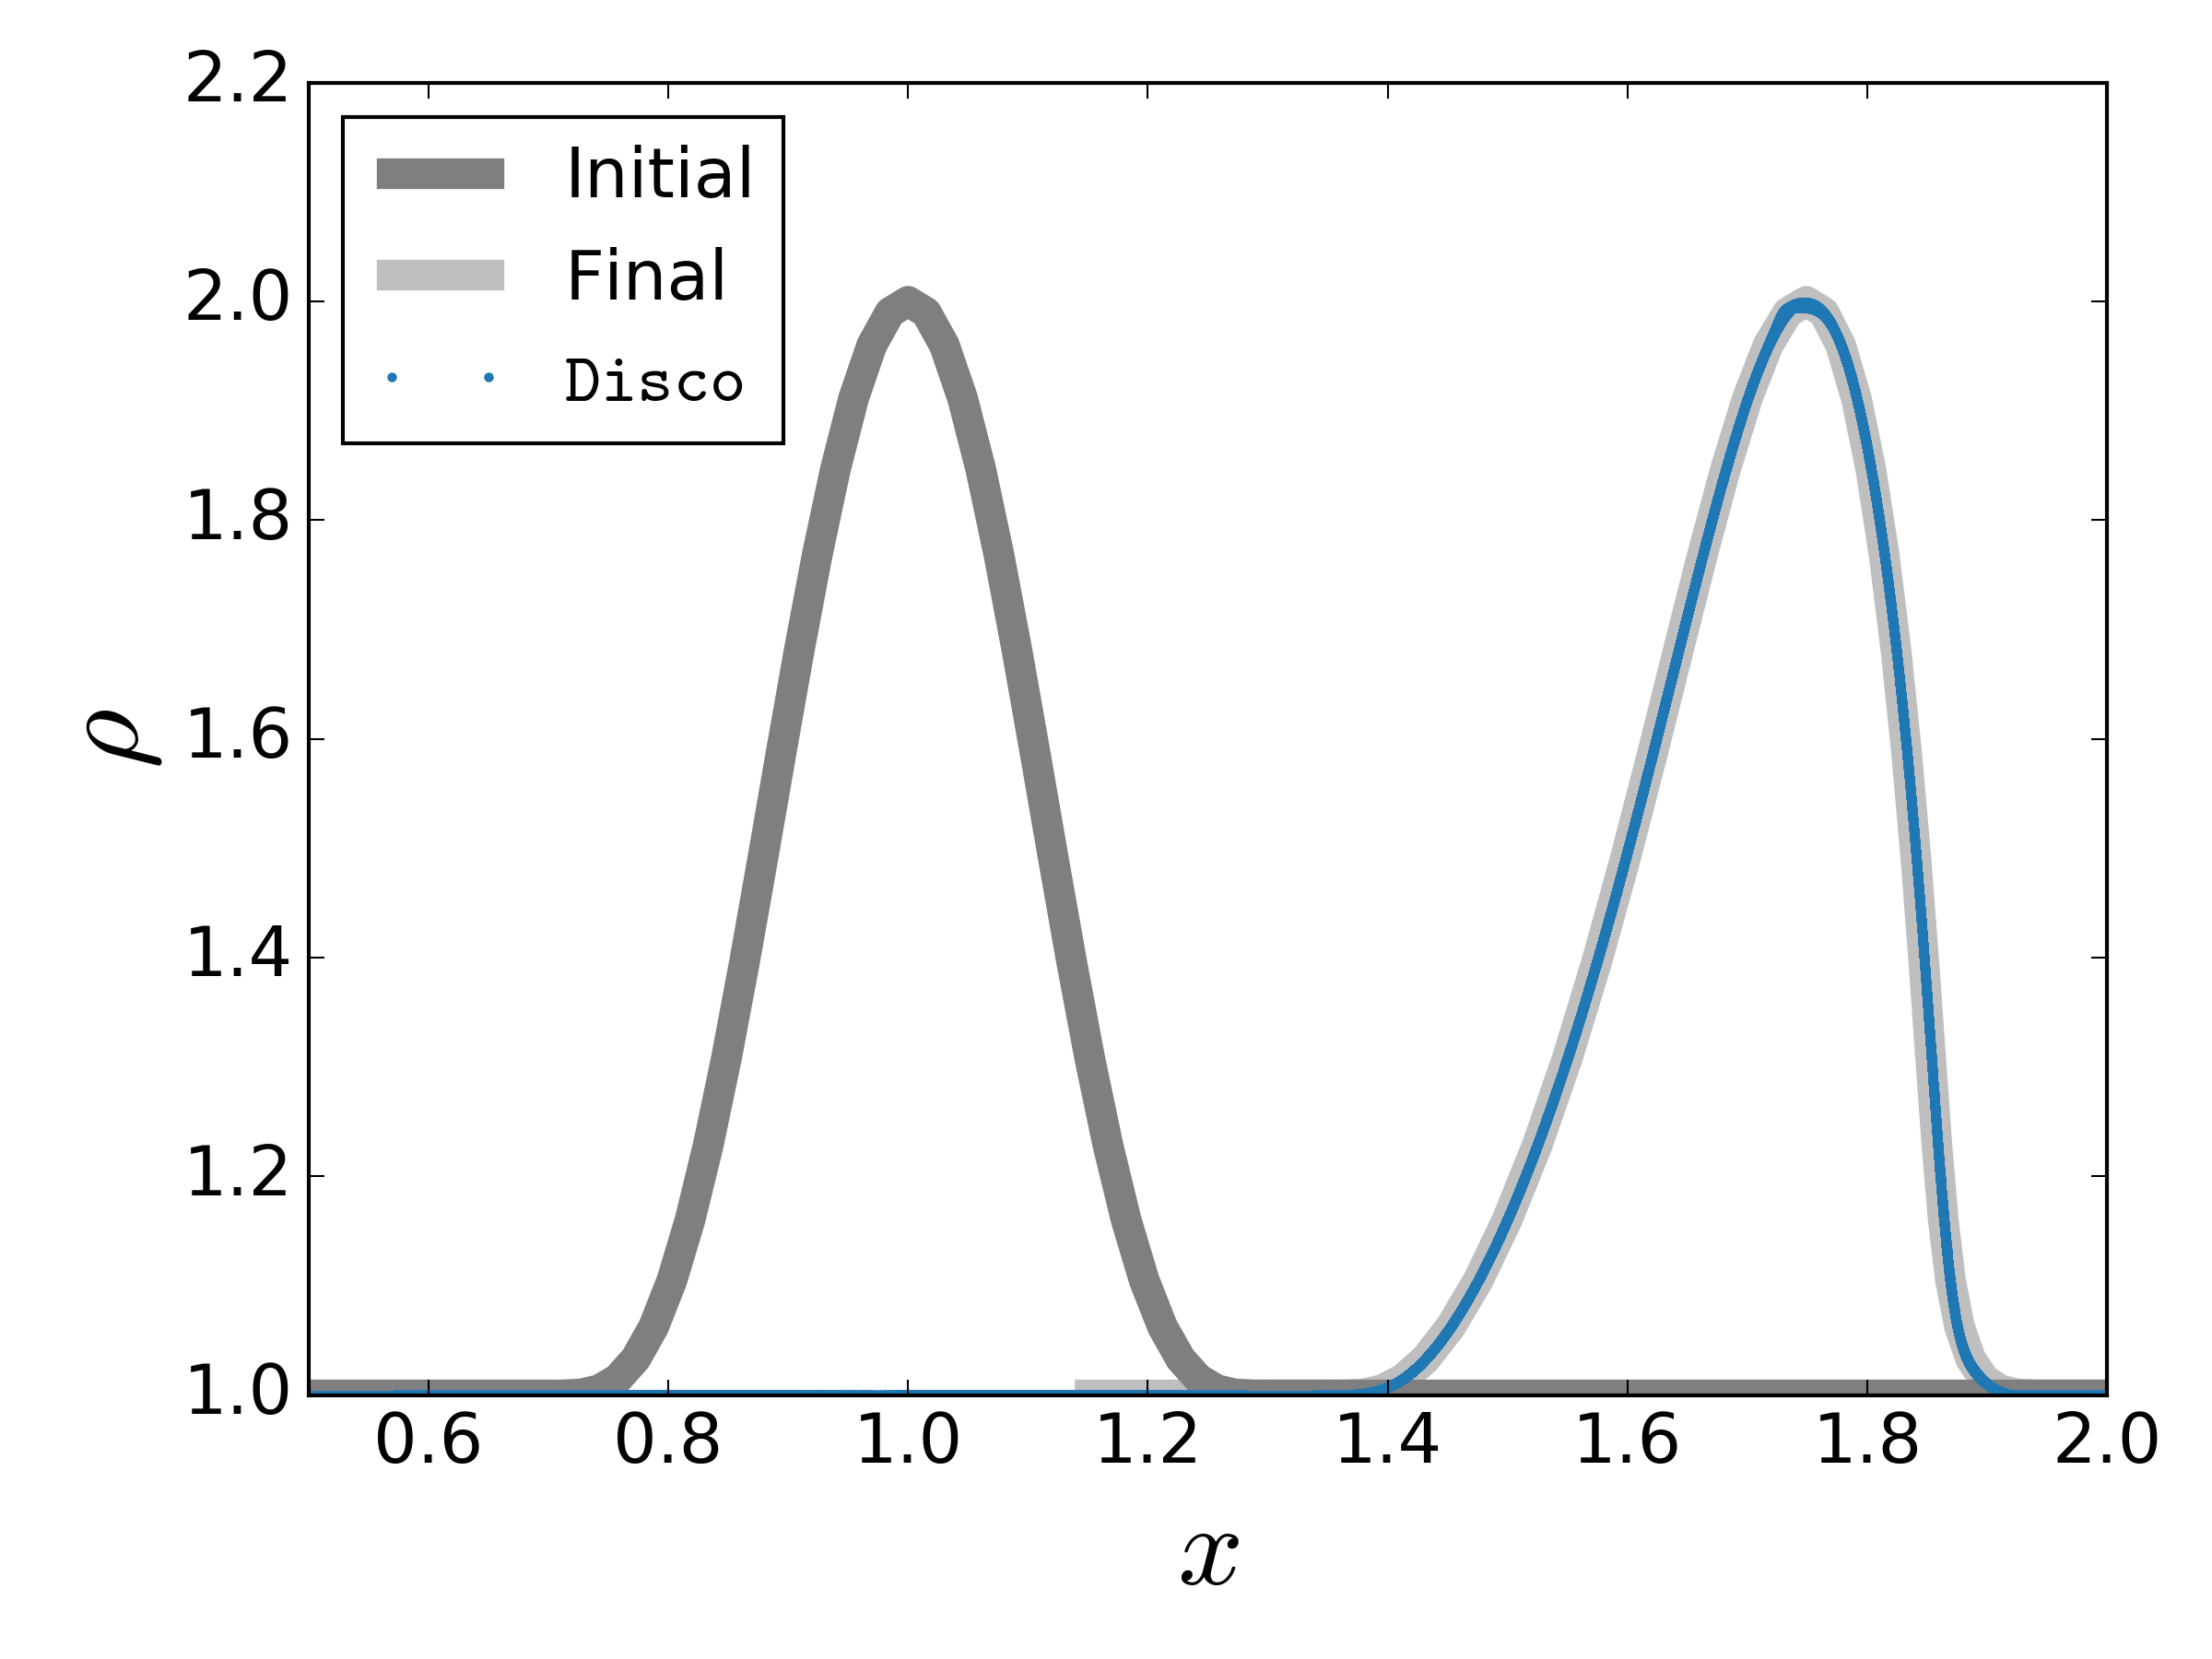
\includegraphics[width=0.65\textwidth]{figures/numerics/isen_1024.png}
\end{center}
\caption{Isentropic wave density $\rho(x)$ at $t=0.8$ for $N_r=1024$ (blue dots), exact solution (grey line), and initial condition (black line).  Despite running obliquely over the cylindrical grid, the wave maintains plane symmetry and matches the exact solution. \figlabel{isen:comp}}
\end{figure}
\begin{figure}
\begin{center}
	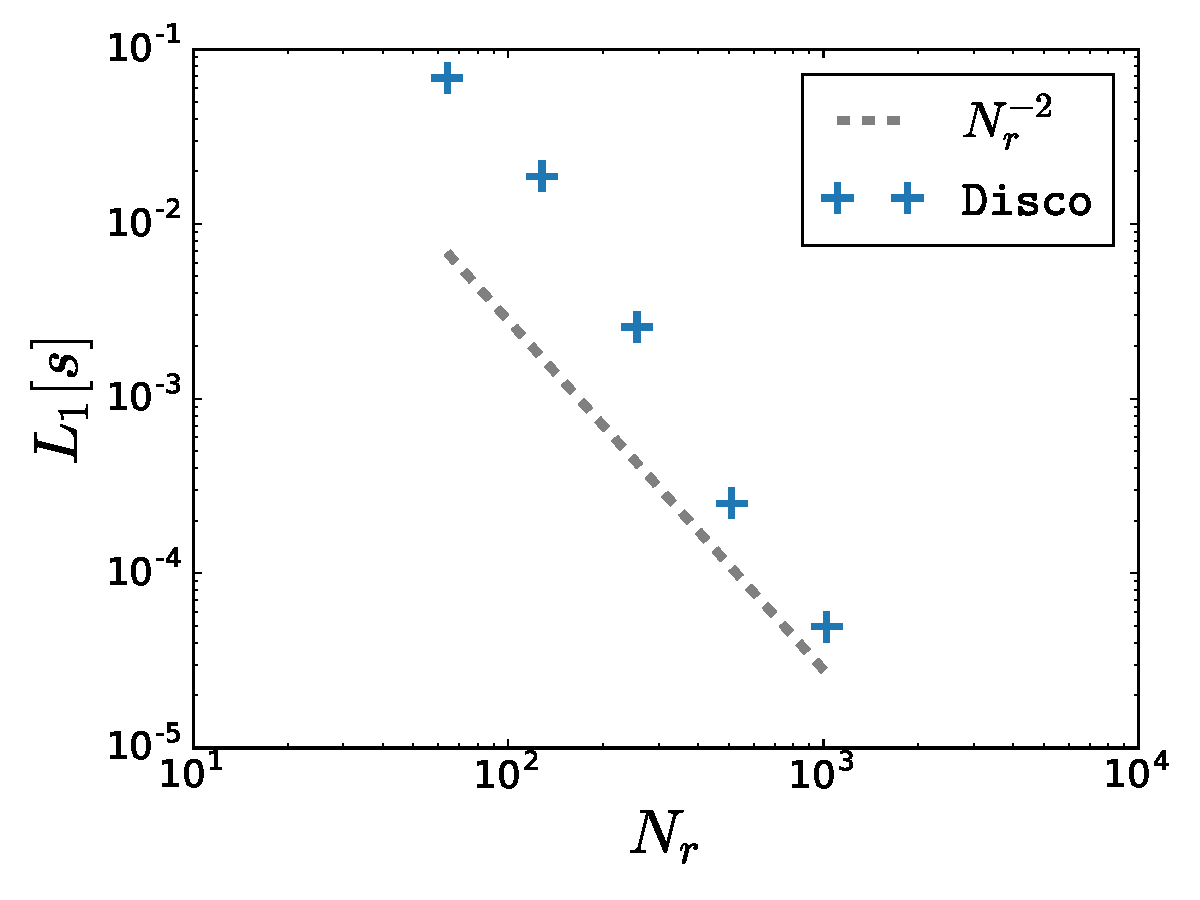
\includegraphics[width=0.65\textwidth]{figures/numerics/isen_conv.pdf}
\end{center}
\caption{$L_1$ error in the entropy $s$ as a function of $N_r$ for the isentropic wave.  The grey dashed line is a visual reference showing the expected convergence rate $N^{-2}_r$.  \figlabel{isen:conv}}
\end{figure}

\fig{isen:comp} shows density at the final time compared with the exact solution.  The agreement with the exact solution is quite good and the lack of dispersion in the data indicates that planar symmetry has been maintained.  To quantify the discrepancy we calculate the $L_1$ error of the entropy:
\begin{equation}
	L_1[s] = \sum_i |s(x_i)-s_0| \Delta A_i\ ,
\end{equation}
where $s(x_i)$ is the entropy of cell $i$, $s_0$ is the ambient (uniform) entropy, $\Delta A_i$ is the area of cell $i$ and the sum is over cells contained in the comparison box.  \fig{isen:conv} plots $L_1[s]$ versus $N_r$ and clearly shows the expected second order convergence.

\subsection{Keplerian Orbit and Inflow}
\sectlabel{test:kep}

This test checks the behaviour of thin accreting disks within the ISCO and demonstrates the efficacy of the energy variable $\tau_U$.  The initial condition is a uniform density disk $\rho(r)=\rho_0$ with uniform pressure $P(r) = P_0 \ll \rho_0$ in the Schwarzschild metric.  The velocity field $u^\mu(r)$ is equal to the geodesic velocity field $U^\mu_{geo}$ defined in \eq{Ugeo}: Keplerian outside the ISCO and smoothly plunging inside.  Outside the ISCO the gas is in a steady state.  Within this ISCO the gas should plunge according to $u^\mu(r)$, which should remain constant so long as $P \ll \rho$.

The analytic solution is given by an advection problem with non-uniform velocity profile.  Define $V = U^r / U^0$ and $F = r \rho V$. Then the continuity equation becomes:
\begin{equation}
	\frac{1}{V}\partial_t F + \partial_r F = 0\ . \eqlabel{kep:adveq}
\end{equation}
For $r > \Risco$ the velocity $V=0$ and $F(r,t)$ is a constant.  For $r < \Risco$ the solution for $F$ is:
\begin{align}
	F(r,t) &= F(r_0, 0)\ , \\
	\text{where } t &= -\int_r^{r_0} \frac{dr}{V(r)}\ .
\end{align}
This gives the solution for $\rho$ and $P$:
\begin{align}
	\rho(r,t) = \frac{r_0 V(r_0)}{r V(r)} \rho_0 \ , \\
	P(r,t) = P_0 \left(\frac{\rho(r,t)}{\rho_0}\right)^\Gam\ .
\end{align}
This one dimensional problem was run with $\rho_0 = 1.0$ and $P_0 = 10^{-4}$ on the domain $r\in[1.5M, 12M]$ in Kerr-Schild coordinates for $\Delta t = 96.344M$, where $M$ is the mass of the black hole.  This time span corresponds to a single orbit at $\Risco = 6M$.  The outer boundary was fixed, and the inner boundary was a hybrid boundary condition with $u^\mu = U^\mu_{geo}$ and $\rho$ and $P$ set to ensure isentropic infall with constant $\dot{M} \propto r\rho u^r$. We used the HLLC Riemann solver, a CFL number of 0.2, a PLM $\theta=1.5$, and $N_r = 384$ radial cells.

\begin{figure}
\begin{center}
	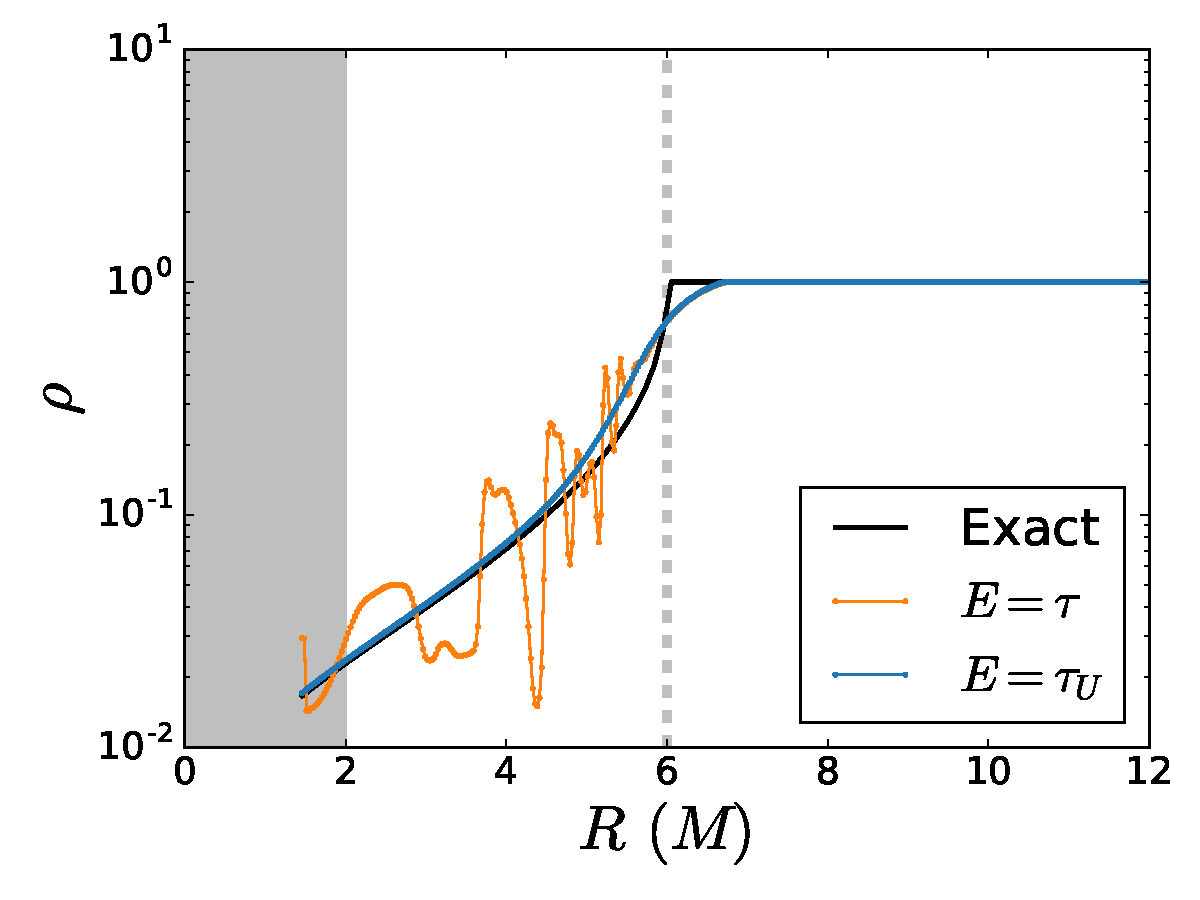
\includegraphics[width=0.6\textwidth]{figures/numerics/kep_rho.pdf}
\end{center}
\caption{Density in the Keplerian flow test at $t\approx96M$.  Exact solution in black, numerical solution with $\tau$ energy variable in orange with dots, numerical solution with $\tau_U$ energy variable in orange with dots.  The $\tau_U$ energy variable is measured in a local Keplerian frame and stably evolves the solution.  Shaded grey area is the event horizon, dashed grey line is the ISCO. \figlabel{kep:rho}}
\end{figure}

\begin{figure}
\begin{center}
	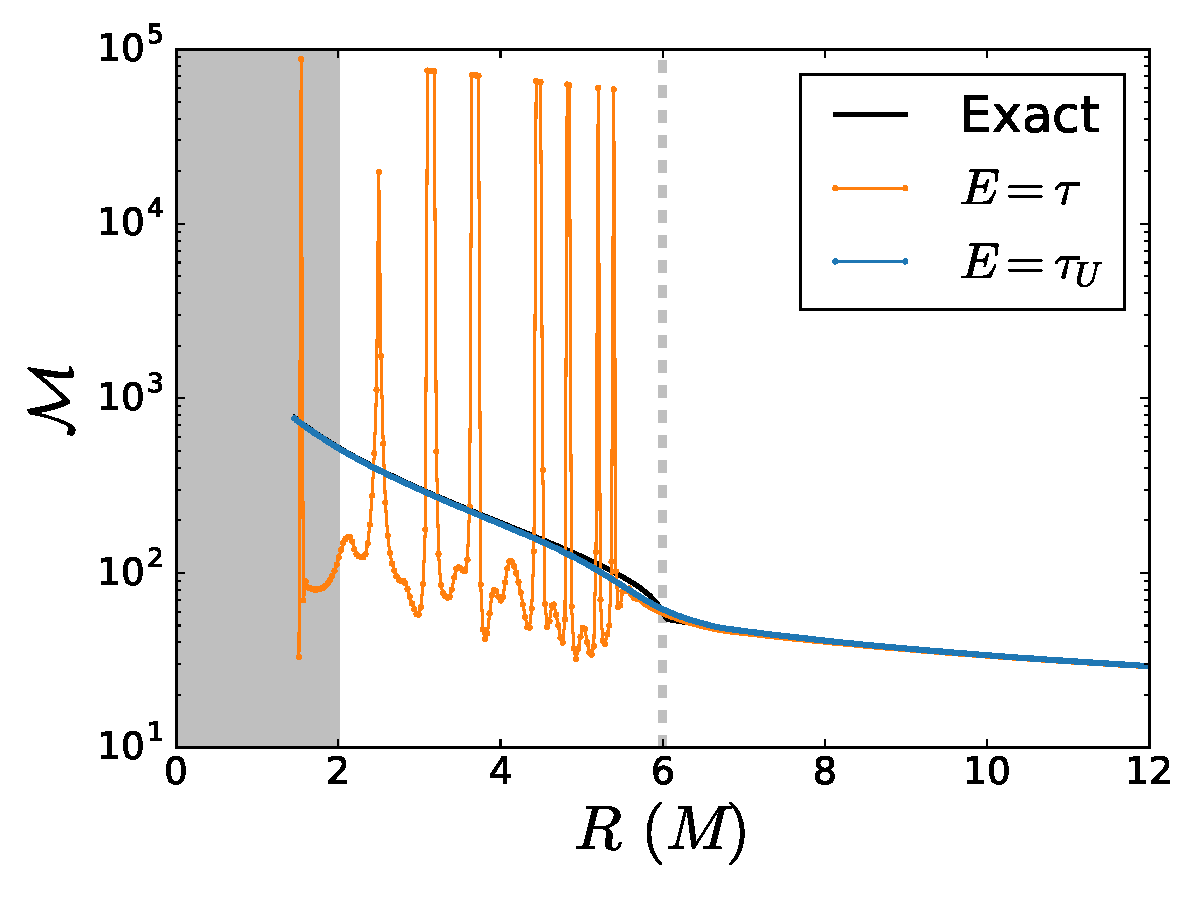
\includegraphics[width=0.6\textwidth]{figures/numerics/kep_mach.pdf}
\end{center}
\caption{Mach number $\mathcal{M} = |u|/c_s$ in the Keplerian flow test at $t\approx96M$, labelling identical to \fig{kep:rho}.   \figlabel{kep:mach}}
\end{figure}

\fig{kep:rho} and \fig{kep:mach} show density $\rho$ and Mach number $\mathcal{M} = |u|/c_s$ in the Keplerian flow test for two energy variables: the standard $\tau$ and our co-moving variable $\tau_U$ using the geodesic frame $U_{geo}$.  The Mach number of this flow is comparable to an x-ray binary or other thin sub-Eddington accretion disks.  The $\tau$ variable completely fails within the ISCO: improperly reconstructed pressures result in wild instabilities which disrupt the density.  The $\tau_U$ variable enables smooth evolution, even up to Mach numbers $\sim 10^3$ where the thermal energy is $\sim 10^{-6} = \mathcal{M}^{-2}$ of the kinetic.  The sharp cusp of the analytic solution $\Risco$ is difficult to resolve as it creates a large pressure gradient which can transport gas inwards.  Realistic disks will always have some form of angular momentum transport, so this is not an issue.

\subsection{Cartesian Shear Flow}
\subsection{Novikov--Thorne Steady State}

As a final test of \grdisco's hydrodynamics solver we find the Novikov--Thorne (NT) $\al$-disk solution in a dynamic calculation \citep{Novikov73}.  We work in the Kerr spacetime in Kerr-Schild coordinates on a radial domain $r \in [1.2M, 100M]$ with $N_r = 128$.  The Kerr parameter is $a_* =0.9$.   This domain crosses the ISCO and ergosphere and has several zones inside the event horizon.  Since the NT solution is vertically integrated and axisymmetric we work in 1D and set $N_\phi = N_z = 1$.  In this setup the density $\rho$ is actually the surface density $\Sigma = \rho H$, where $H$ is the disk scale height.  Similarly $P$ is the vertically integrated pressure.  We use $\al$-viscosity and set $\al = 0.1$.  

To balance the viscous heating we include a cooling source term corresponding to a disk blackbody with opacity due to electron scattering:
\begin{equation}
	\dot{Q} = \frac{8}{3}\frac{ \sig_{\rm SB}T^4}{\ka_{\rm es} \Sig}\ . \eqlabel{BBcooling}
\end{equation}
In \eq{BBcooling} $\sig_{\rm SB}$ is the Stefan-Boltzmann constant and $\ka_{\rm es} = 0.4$ cm\textsuperscript{2}/g is the electron scattering opacity.  This is incorporated by modifying the conservation of energy-momentum equation as:
\begin{equation}
	\nabla_\mu T^{\mu\nu} = - \dot{Q} u^\nu\ .
\end{equation}

The initial condition is the NT solution for $r>30M$ with a set accretion rate $\dot{M}$, we set $M = 10 M_\odot$ and $\dot{M} = 10^{-4} \dot{M}/y$.  Inside $30M$ the solution has uniform density and pressure.  The simulation is run for $t = 10^5 M$ with $\CFL=0.2$, PLM $\theta=1.5$, HLL Riemann solver, adiabatic index $\Gam = 5/3$, and energy frame velocity $U^\mu_{\rm geo}$. 

\begin{figure}
\begin{center}
	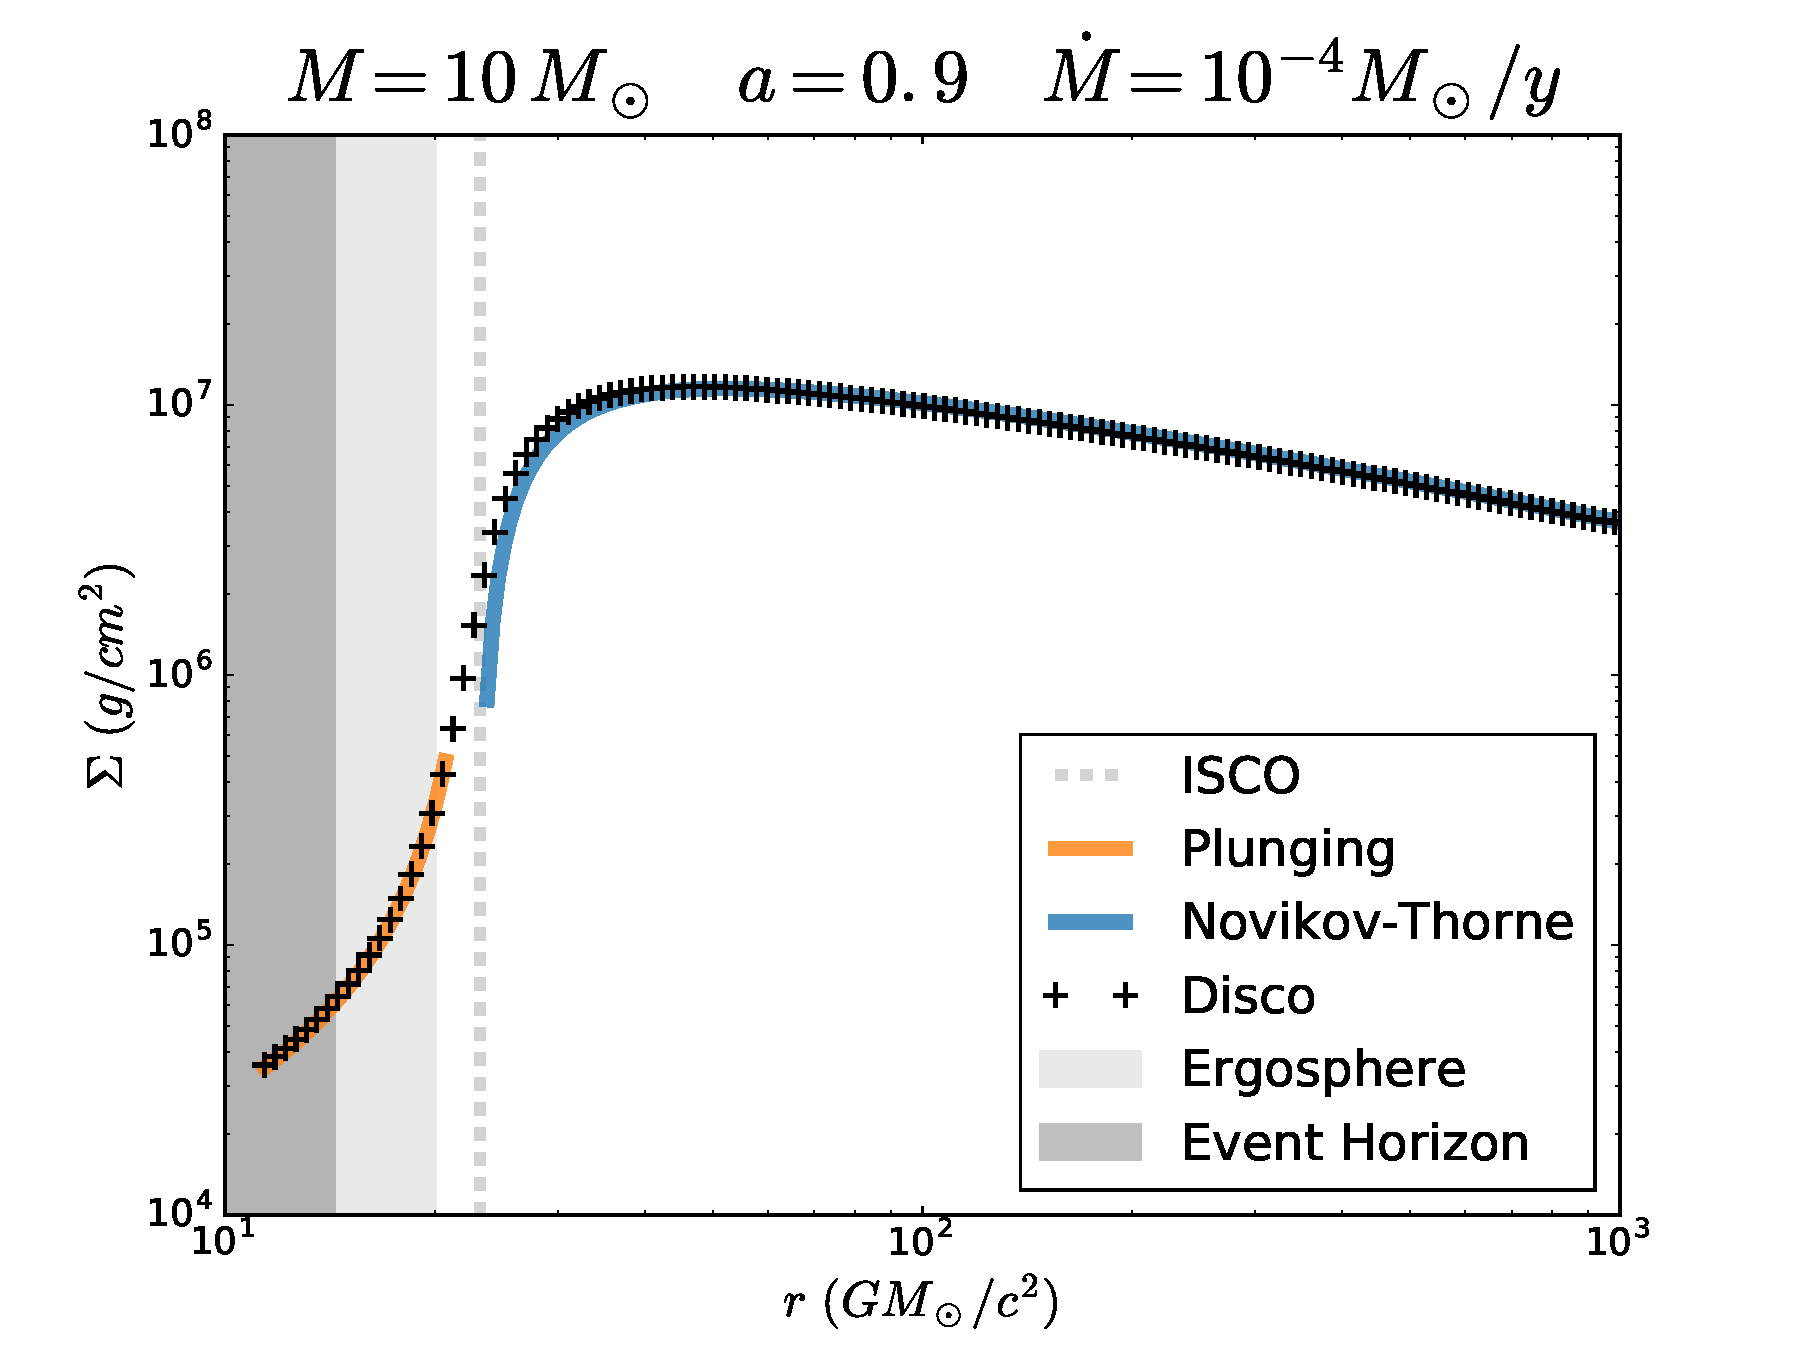
\includegraphics[width=0.65\textwidth]{figures/numerics/nt_sig.pdf}
\end{center}
\caption{Surface density in steady state with $\al$ viscosity and cooling in the Kerr metric.  Disco data in black crosses, Novikov--Thorne solution in blue, isentropic plunging in orange.  The grey dashed line denotes the ISCO, the light grey shading the ergosphere, and the dark grey the black hole interior.  \figlabel{nt:sig}}
\end{figure}

The inner disk quickly accretes as in the Keplerian inflow test, but over time is refilled due to viscous stresses.  Viscous heating is balanced by radiative cooling and a steady state is reached, shown in \fig{nt:sig}.  The density profile matches the Novikov--Thorne solution outside the ISCO and smoothly continues into the horizon.  Inside the ISCO the solution is well approximated by a ``plunging'' solution characterized by $u^\mu = U^\mu_{\rm geo}$, $\dot{M}$ constant, and $P / \Sig^\Gam$ constant.  

The NT solution by construction assumes the torque $\tau^r_\phi(r=\Risco) = 0$.  This allows for simply-parameterized algebraic solutions but causes the profile to diverge at $\Risco$.  Our dynamic calculation naturally finds a small torque at the ISCO, extending the NT solution smoothly into the horizon.

\begin{figure}
\begin{center}
	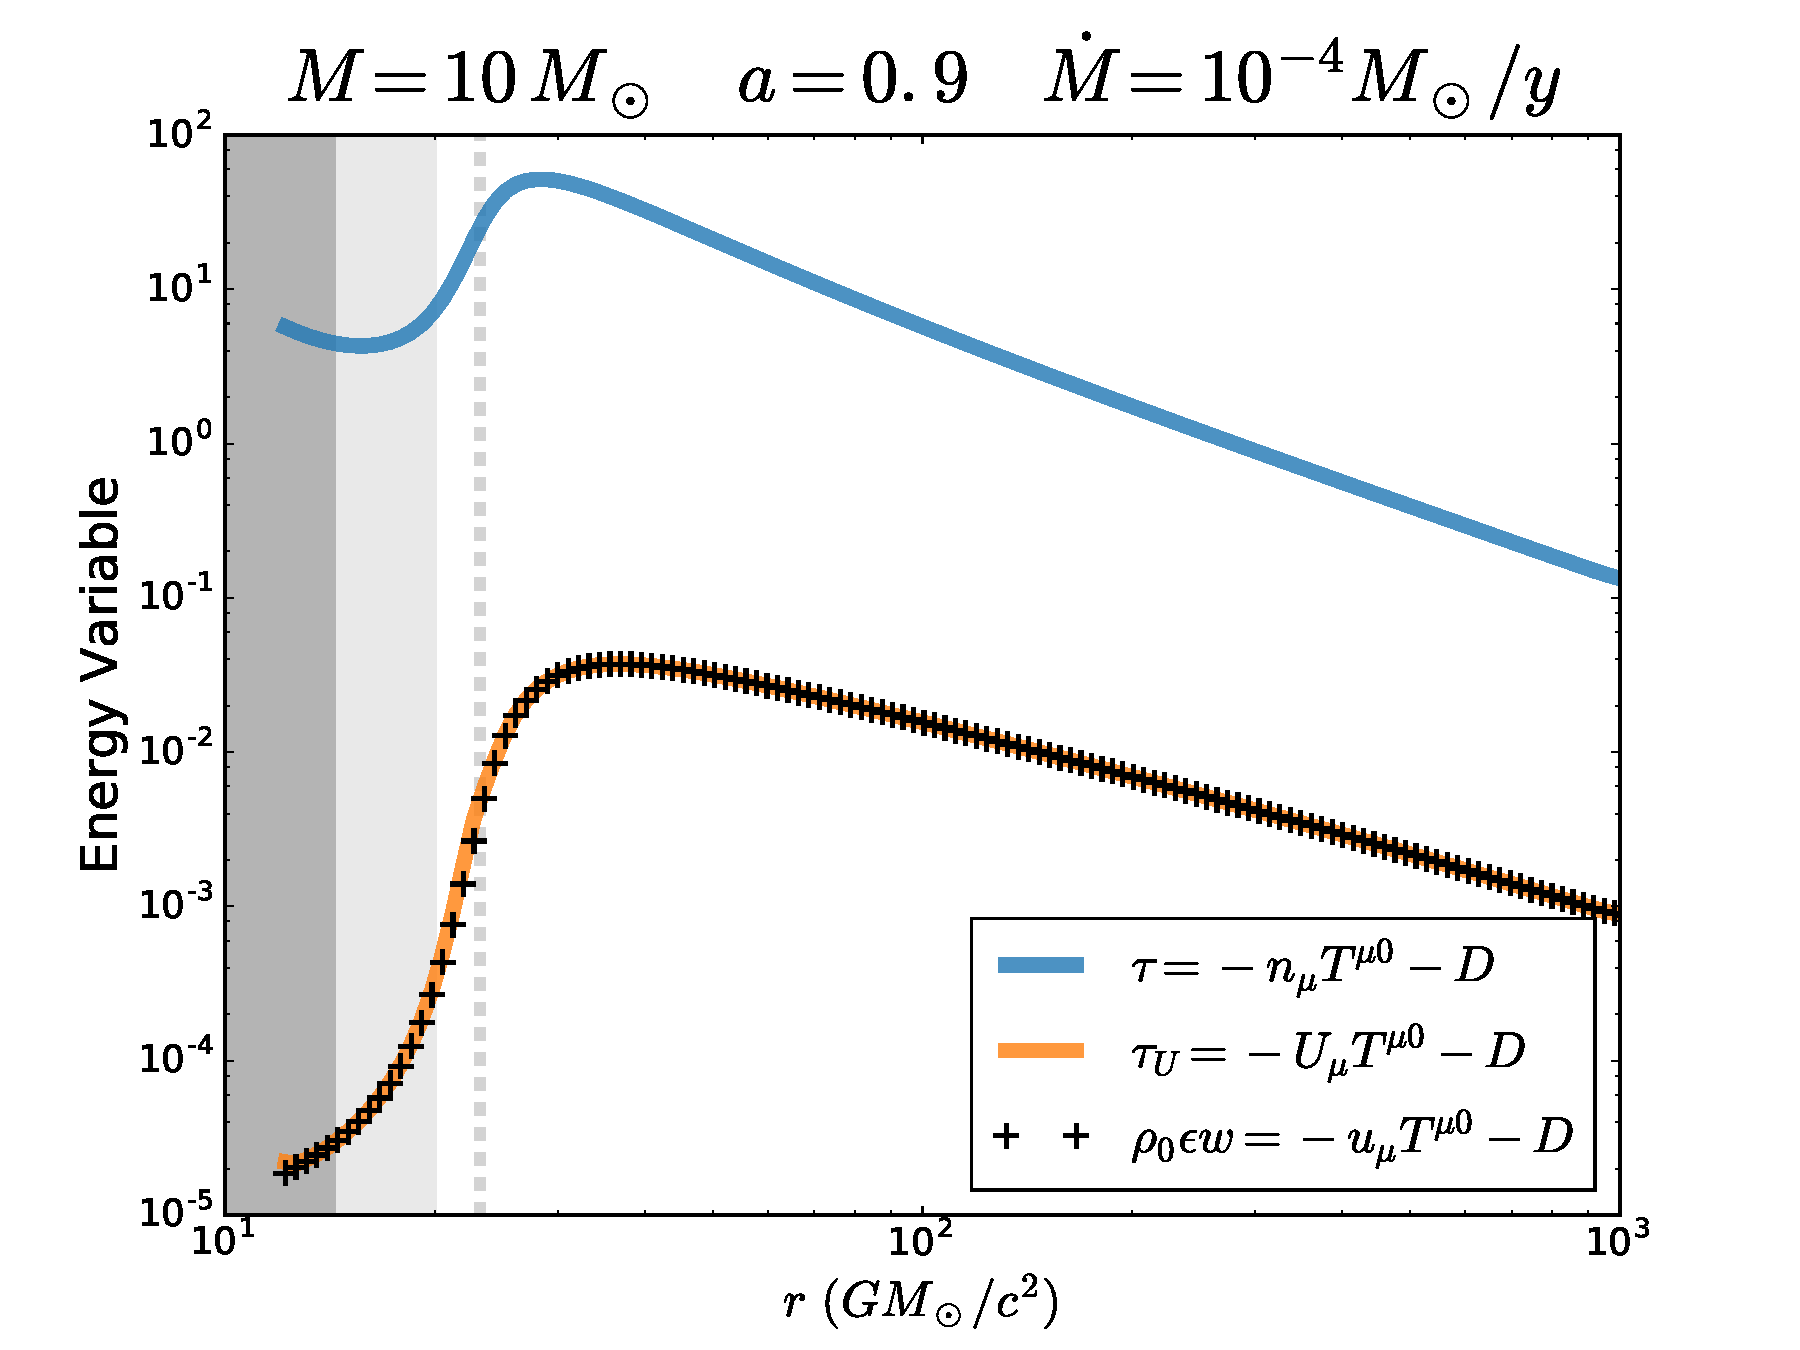
\includegraphics[width=0.65\textwidth]{figures/numerics/nt_eps.pdf}
\end{center}
\caption{Energy variables for the dynamic Novikov--Thorne solution. Standard variable $\tau$ in blue, our co-moving variable $\tau_U$ in orange, and the internal energy density in black crosses.  Other markings identical to \fig{nt:sig}.  \figlabel{nt:eps}}
\end{figure}

For illustration \fig{nt:eps} shows the energy variables $\tau$ and $\tau_U$ compared to the lab frame internal energy density $\rho \eps u^0$.  We see near agreement between the internal energy and $\tau_U$ and a vast difference with $\tau$, which is several orders of magnitude larger.  Truncation errors of the order $10^{-6}$ in the energy can easily swamp out the internal energy entirely in the inner disk.  Note that for realistic x-ray binaries the accretion rate used here is quite large.  Realistic binaries have smaller accretion rates, higher mach numbers, and would produce an even larger discrepancy between $\tau$ and the internal energy.  

%\subsection{Neutrino Dominated Accretion Flow Steady State}
\subsection{Magnetic Field Loop Advection}
%\subsection{Magnetic Blastwave}
\subsection{Linear MRI}

%%%%%%
% Summary %
%%%%%%

\section{Summary}
\sectlabel{summary}

We have introduced \grdisco, a new three dimensional GRMHD code that utiliizes a moving, shearing mesh.  The mesh motion greatly lowers the numerical dissipation while allowing for significantly longer time steps.  We have demonstrated \grdisco's performance on a number of test problems which show its accuracy and the utility of its advanced Riemann solvers.  \grdisco is massively parallel and available freely online at \url{https://github.com/geoffryan/Disco.git}.

\section{Chapter Acknowledgements} \sectlabel{acknowledgements}

We thank Brian Farris for many fruitful conversations and his work on Newtonian \disco.  

